% TODO: MOSTRAR FOTO DEL BOTON PINGPONG

\documentclass{article}
\usepackage[utf8]{inputenc}
\usepackage[spanish]{babel}
\usepackage[draft]{graphicx}	%Si se quiere compilar con las imagenes
% \usepackage[draft]{graphicx}	%Si NO se quiere compilar con las imagenes porque tarda mucho
\usepackage{graphics, float, fancyhdr, titling, caption, subcaption}
\usepackage{listings}
\usepackage[a4paper, total={6in, 9.5in}]{geometry}
\usepackage{fancyhdr}
\usepackage{hyperref}   %para que funcione addcontentsline debe ser la ultima que se cargue
\usepackage{amsmath}
%\setcounter{secnumdepth}{-2}       %Poner solo esto si no se quieren numero delante de las secciones y niveles inferiores.

\renewcommand{\footrulewidth}{0.4pt}
\title{

\includegraphics[width=1.75in]{imagenes/UGR-Logo.png} \\
\vspace*{1in}
\textbf{Memoria de la práctica 3} \\
Animación por Ordenador \\
\vspace*{0.5in}}
\author{Andrés Merlo Trujillo \\
andresmerlo@correo.ugr.es \\
77147239H \\ 
\vspace*{0.5in} \\
E.T.S. de Ingenierías Informática y de Telecomunicación \\
\textbf{Universidad de Granada}} \date{\today}

\hypersetup{
    colorlinks=true,
    linkcolor=black,
    citecolor=black
}

\renewcommand\maketitlehooka{\null\mbox{}\vfill}
\renewcommand\maketitlehookd{\vfill\null}

\begin{document}
\begin{titlingpage}
\maketitle
\end{titlingpage}

\tableofcontents

\newpage

\pagestyle{fancy}   %a partir de comienza el header (se salta el indice y portada)
\fancyhead[L]{Andrés Merlo Trujillo}
\fancyhead[R]{Animación por Ordenador}
%\section{Ejercicio 1}
%\begin{figure}[H]
%    \centering
%    \includegraphics[width=\textwidth]{imagenes/passwdfile.png}
%    \vspace{10pt}
%    \footnotesize{Fuente: https://...}
%\end{figure}

% \begin{figure}[H]
%     \centering 
% 	\begin{subfigure}[t]{0.48\textwidth}
% 	    \centering
% 	    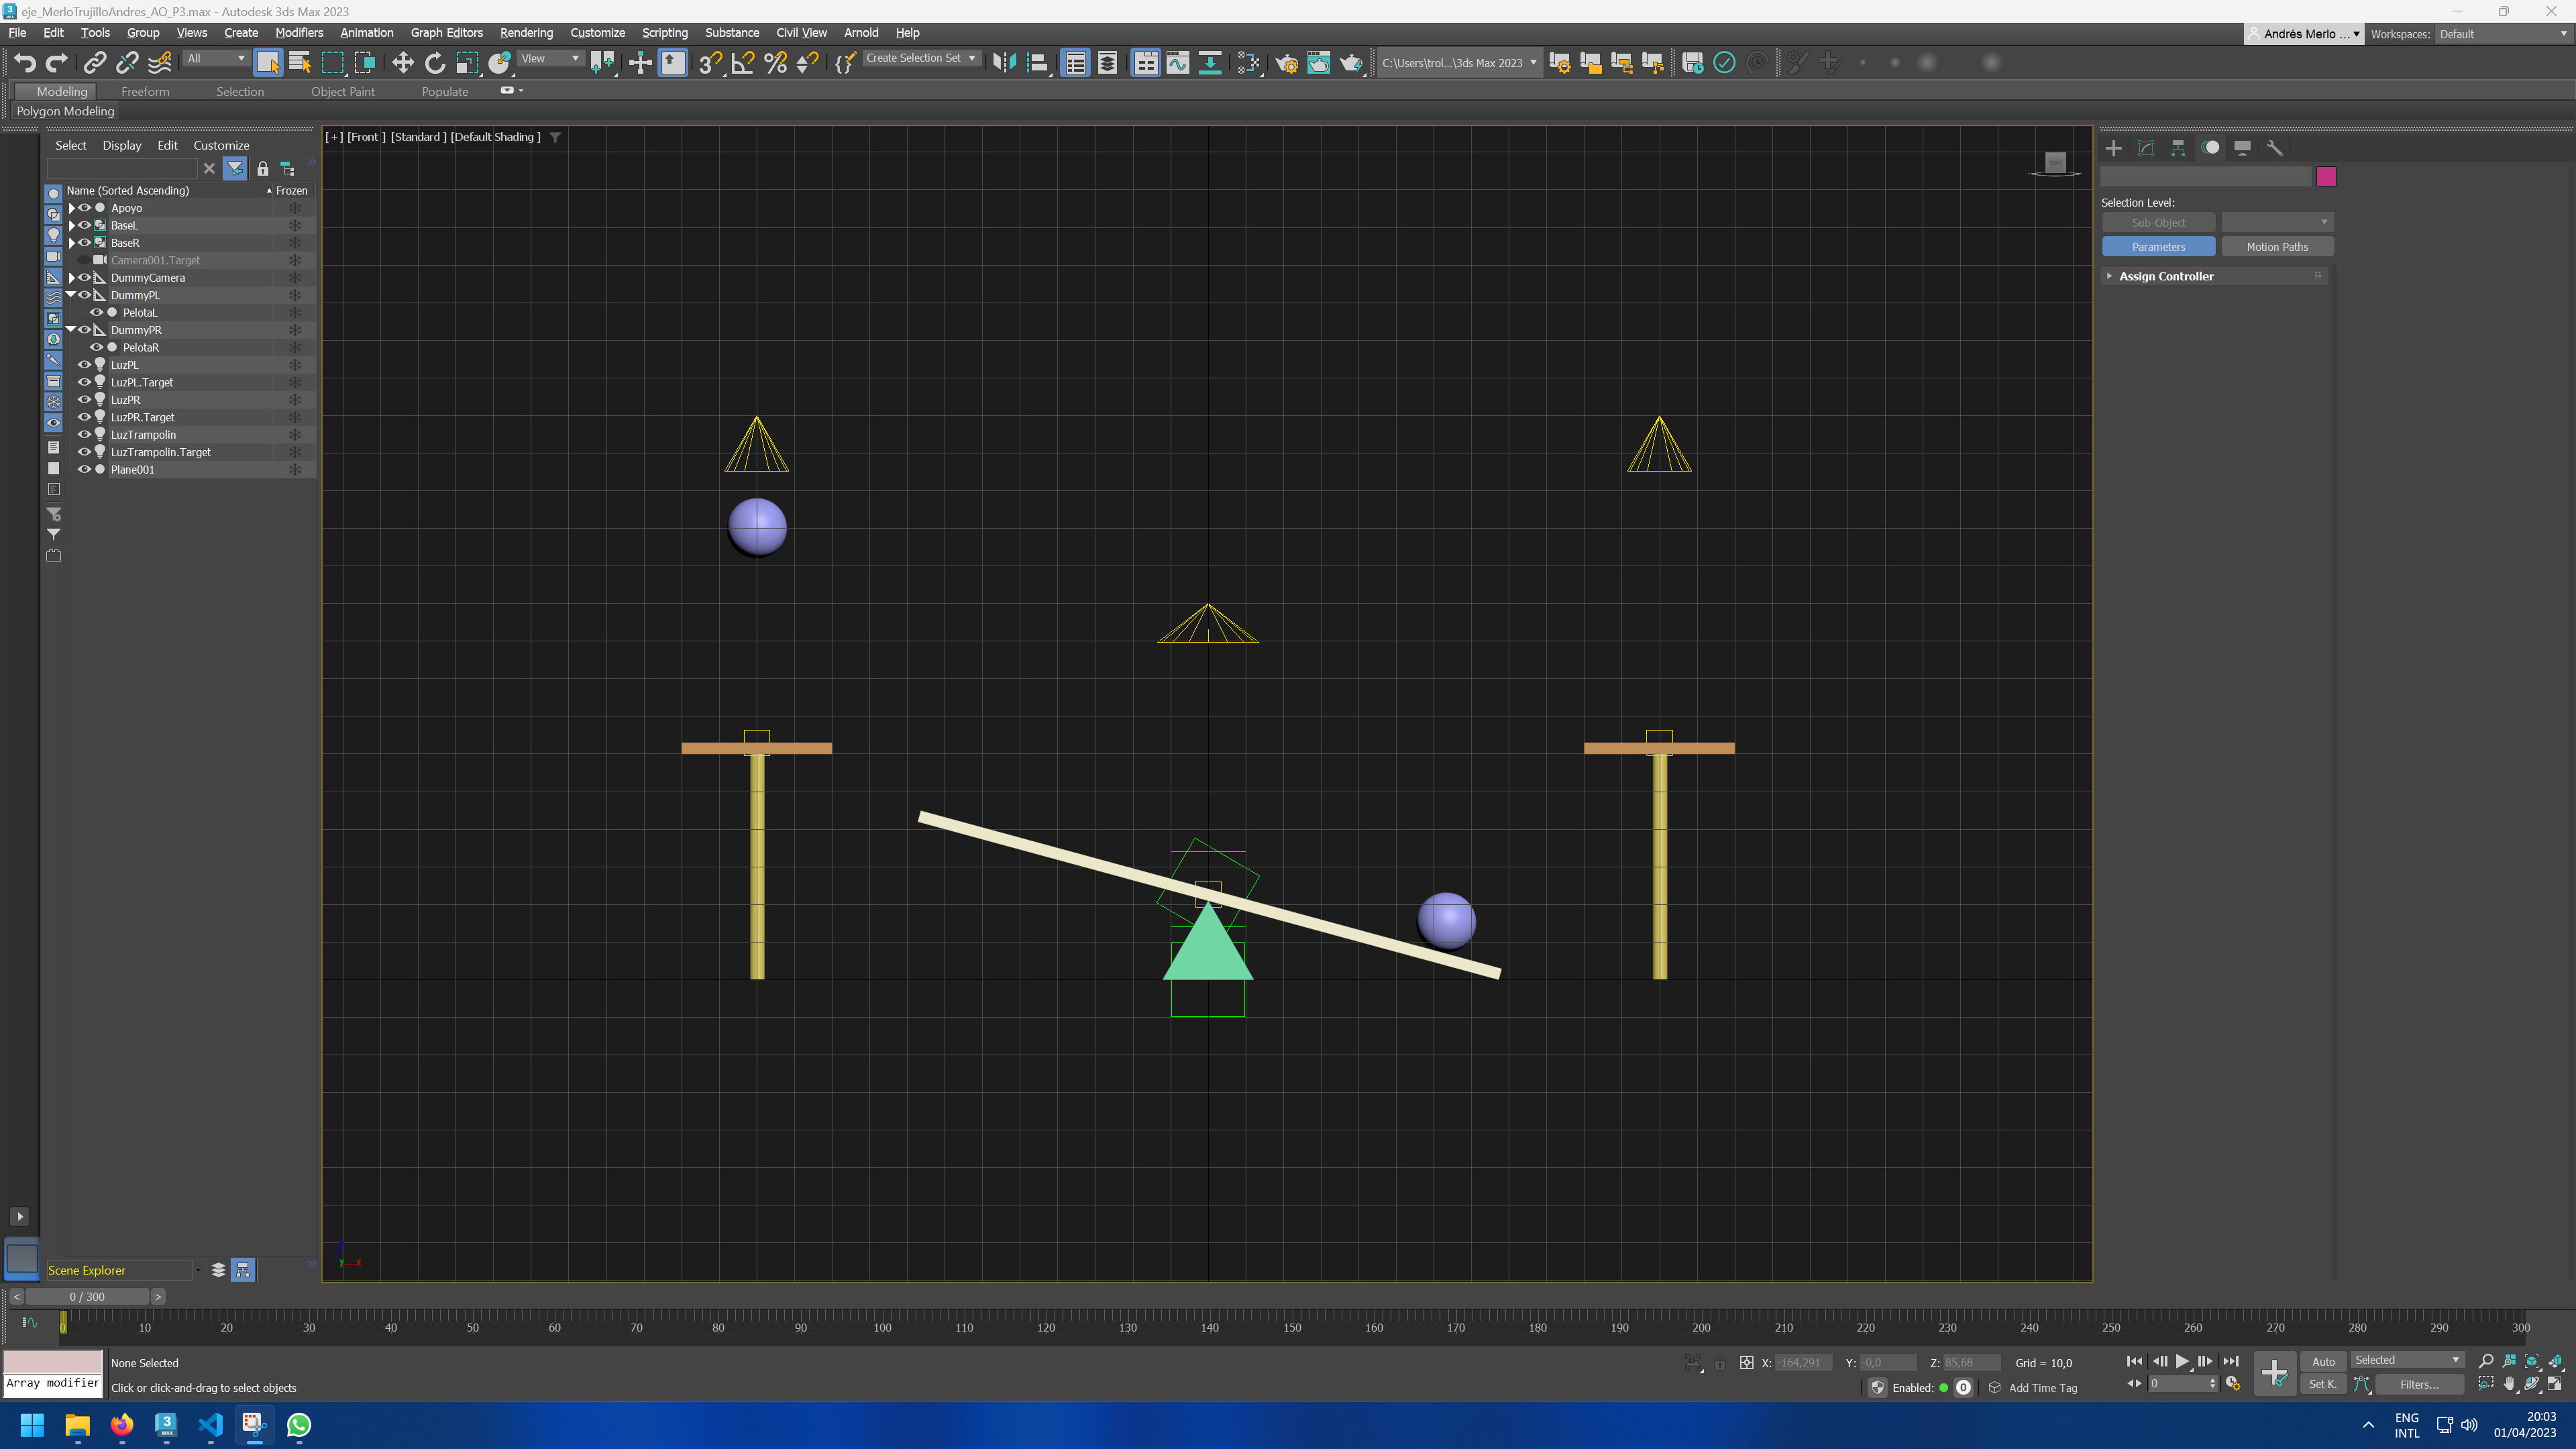
\includegraphics[width=\textwidth]{imagenes/Ejercicio 1/keyframes/0.png}
%         \caption{Pelotas en el instante 0.}
%     \end{subfigure}
%     \hfill
%     %\par\bigskip %si se desea dejar un margen entre la imagen de arriba y de abajo
% 	\begin{subfigure}[t]{0.48\textwidth}
% 	    \centering
% 	    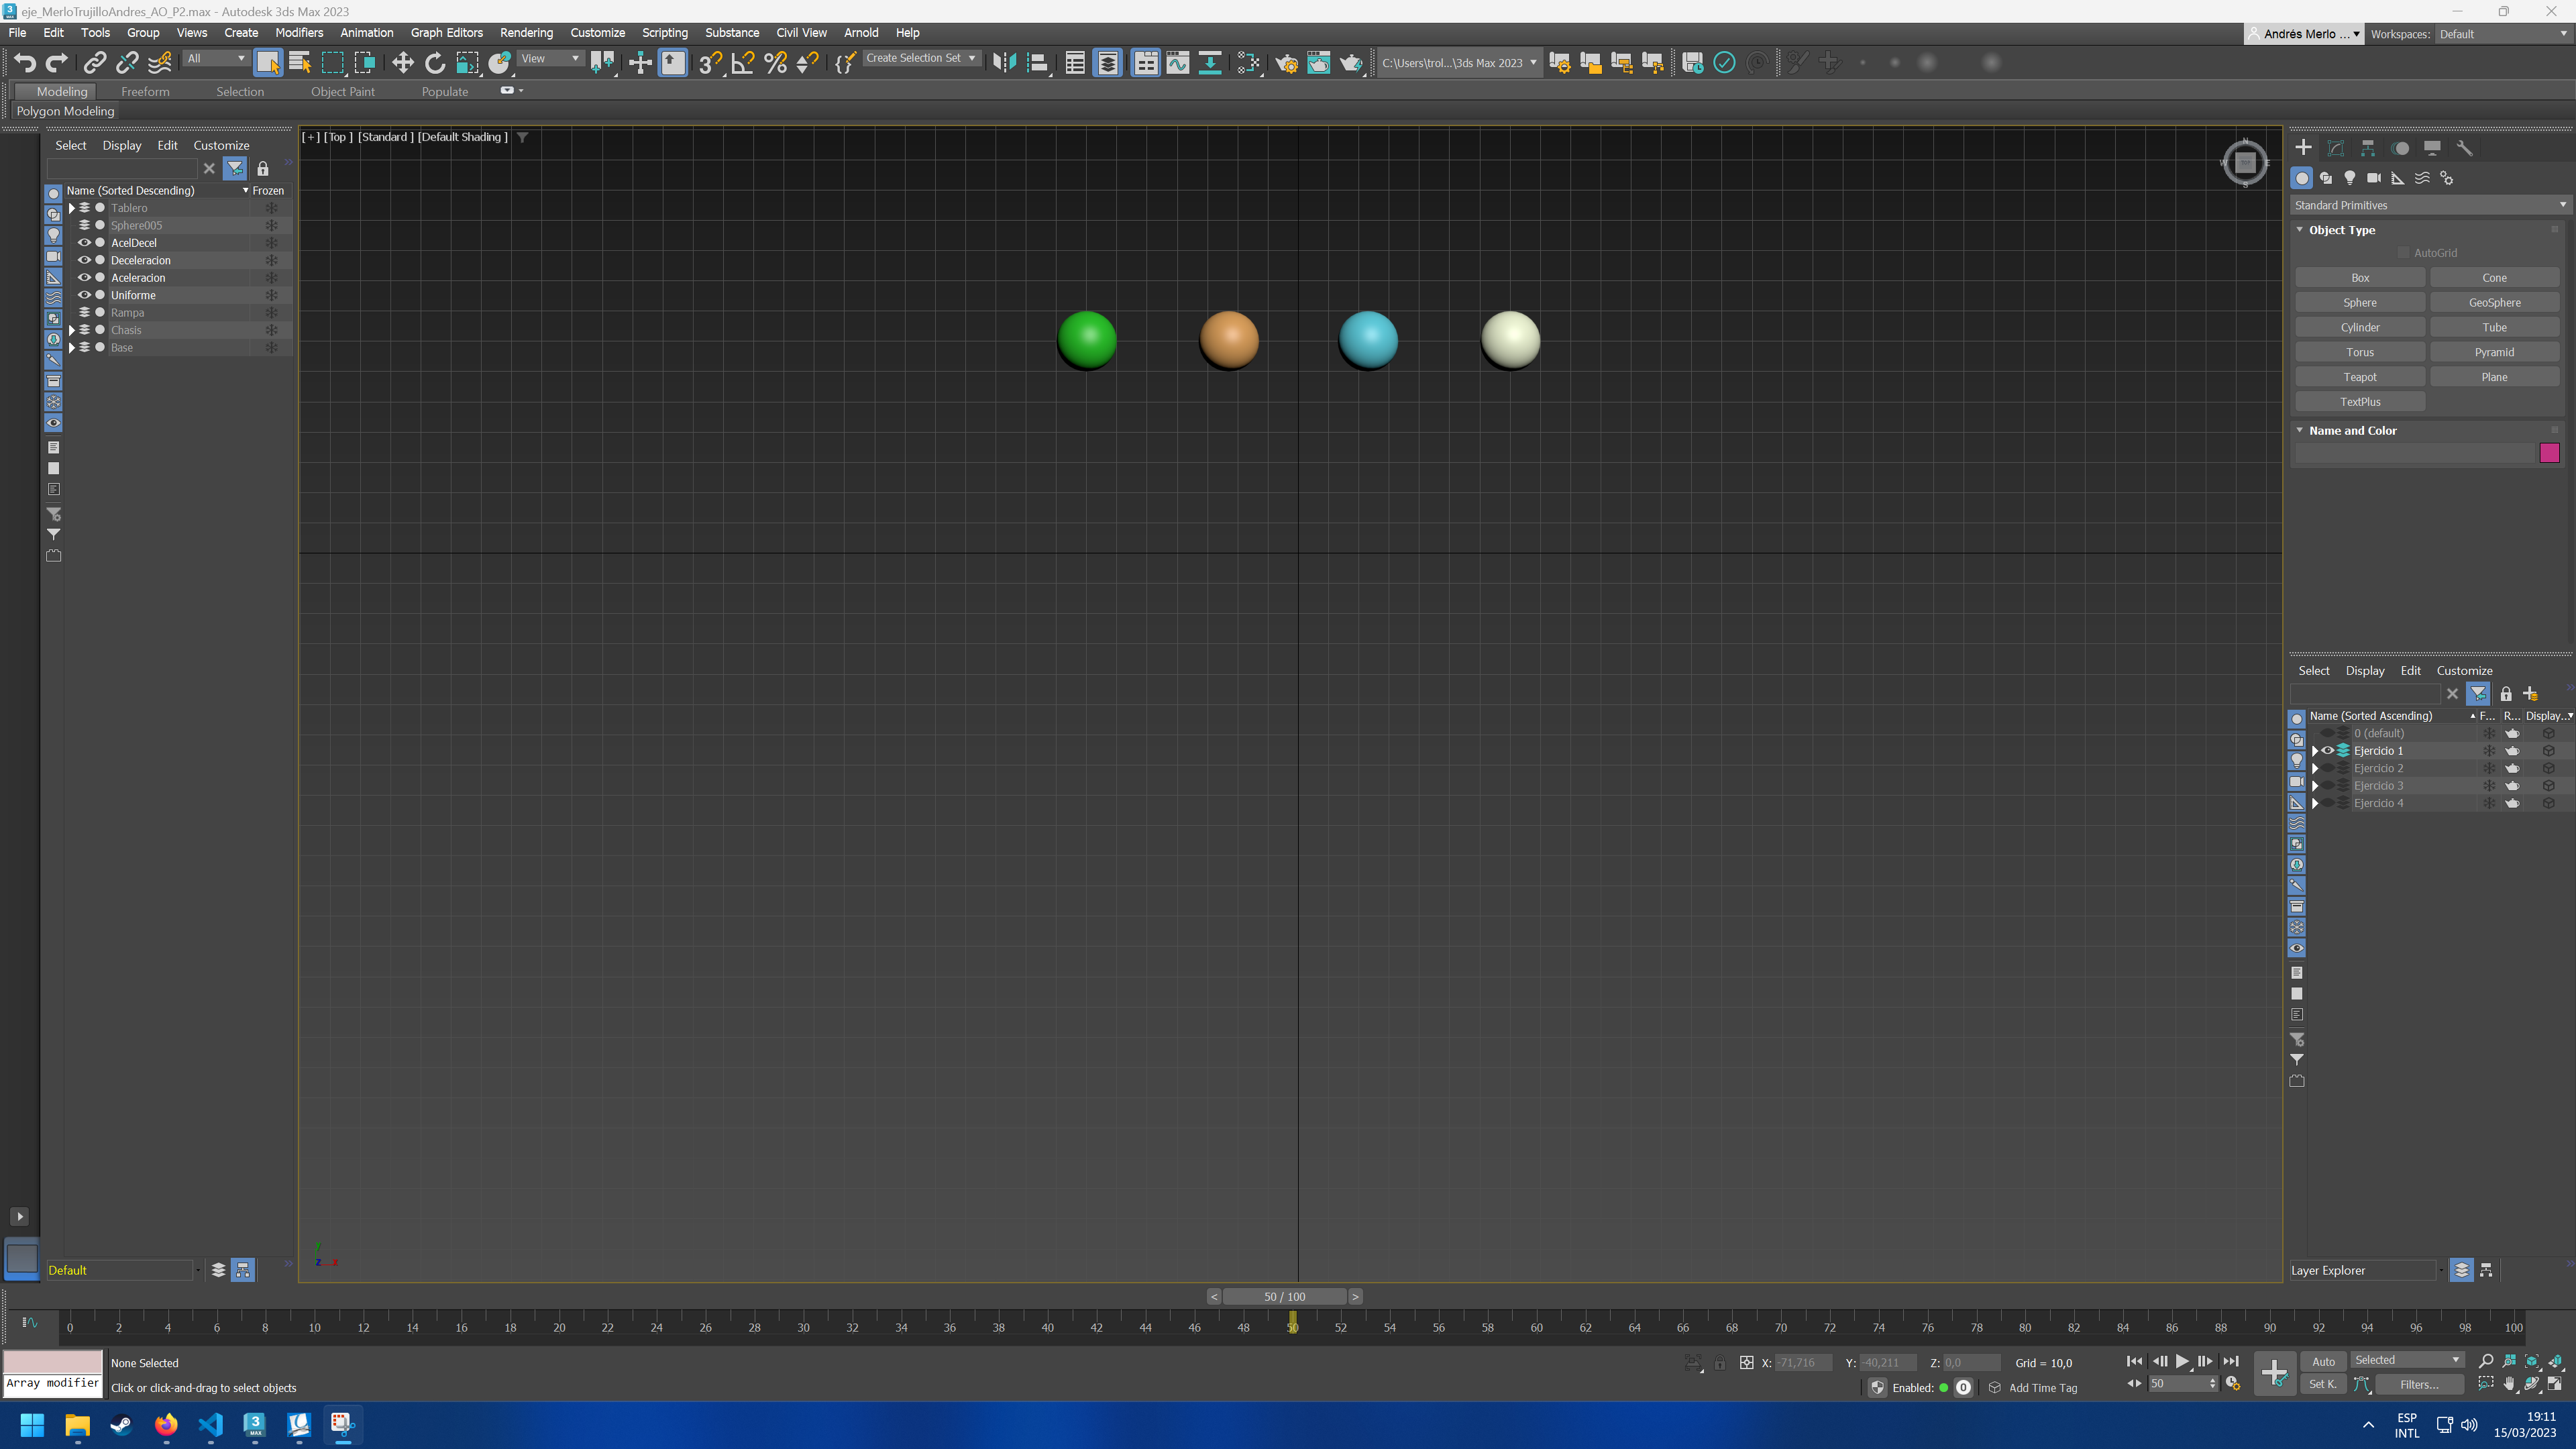
\includegraphics[width=\textwidth]{imagenes/Ejercicio 1/keyframes/50.png}
%         \caption{Pelotas en el instante 50.}
%     \end{subfigure}    
% \end{figure}


\section{Introducción}
% rescribir
En esta práctica se pide animar un conjunto de pelotas, que rebotan y caen a un balancín, haciendo que la otra rebote y caiga en una plataforma. También se debe animar un conjunto de luces que iluminará la parte de la escena que está en movimiento actualmente y una cámara, que rotará alrededor de la escena.

Todo lo mencionado anteriormente se debe \textit{loopear} de forma invertida, de manera que cuando acabe la animación vuelva a realizarse, pero al revés, comenzando por el final y acabando por el principio.

En esta memoria voy a dividir cada una de las partes que he realizado en secciones, las cuales se encontrarán a continuación.

\section{Número de fotogramas}

% rescribir
En la práctica se pedía que la animación durase 5 segundos, y otros 5 segundos haciendo la animación inversa. 

En mi caso, he usado 30 fotogramas por segundo, los que pone por defecto 3ds Max. Por tanto los cálculos para obtener lo números de fotogramas necesarios son los siguientes:


$30 \text{ fps} \times 2 \times 5 \text{ segundos} = 300 \text{ fotogramas} $

Cabe destacar que la animación debe acabar en el instante 150, para dar paso a su inversa y se complete.

\section{Composición de los objetos compuestos}

Los distintos objetos de la escena se han construido de la siguiente forma:

\begin{itemize}
    \item \textbf{Trampolín: }Se ha utilizado un cubo achatado y estirado para hacer la tabla y para el punto de apoyo se ha usado un cilindro con un circulo de 3 lineas, haciendo que sea un triangulo.
    
    Además, he modificado el pivote del tablero para que se encuentre justo en la unión del punto de apoyo con la tabla, para que gire de manera realista.

    Cabe destacar que he realizado una jerarquia en la que el punto de apoyo es el padre.

    \item \textbf{Bases: }Para las bases he utilizado un cubo achatado y un cilindro para el soporte, uniendo ambos en un grupo.
\end{itemize}


\section{Animación de la escena}

La animación la he realizado algo distinta a la que se pedía en el guion, ya que le comenté al profesor que el resultado era muy lento y me dijo que podía añadir algunos rebotes antes de comenzar la animación pedida. Para dar simetría, he animado dos rebotes al principio de la animación y al final. 

Además, como se pide seguir una forma Ping-pong cuando esté fuera de los \textit{keyframes} animados, va a haber \textit{keyframes} que se van a repetir en el instante 0 y 150; es decir, que no va a haber cambio con el siguiente o el anterior. Esto es necesario, ya que hay animaciones que no duran lo mismo, como el balancín, que su animación es más corta y si no se hiciera daría como resultado un giro prematuro del trampolin.

\bigskip

% rescribir
Para animar el movimiento de las pelotas que realizan en el balancín, he usado un objeto \textit{Dummy} con centro en la superficie del balancín y siendo padre de la pelota en la jerarquia; es decir, en la misma superficie donde las pelotas se encuentra.

% foto de los dummies

Además, para que la trayectoria que realicen no se vea afectada por la rotación del \textit{Dummy}, este se debe encontrar sin ninguna rotación en el momento en el que salen/entran al trampolín.

\bigskip

Ahora bien, como puede haber confusión sobre los distintos \textit{keyframes} para los objetos de la escena, voy a dividir cada objeto junto a su \textit{Dummy}, si lo tiene, en subsecciones:

\subsection{Pelota de la izquierda}

Los \textit{keyframes} para la pelota de la izquierda son:

\begin{itemize}
    \item \textbf{Instante 0: }La pelota se encuentra sobre su base, a cierta altura de la misma para realizar varios rebotes.
    \item \textbf{Instante 14: }La pelota se encuentra sobre su base, tocando la superficie de la misma, debido a la caida de la pelota.
    \item \textbf{Instante 26: }La pelota se encuentra en el aire, con la misma altura que en el instante 0. Esto lo hago asi para que la animación ping-pong funcione de manera mas o menos realista.
    \item \textbf{Instante 38: }La pelota se enceutnra sobre la superficie de la base, esta vez lista para saltar al trampolin.
    \item \textbf{Instante 48: }La pelota se encuentra en su punto mas alto del salto hacia el trampolin.
    \item \textbf{Instante 58: }La pelota ha caido y se encuentra sobre el trampolin.
    \item \textbf{Instante 150: }Exactamente igual que el instante anterior, para que la animacion se pueda rtepetir correctamente.
\end{itemize}

Las curvas de animación para la pelota son:

\begin{figure}[H]
   \centering
   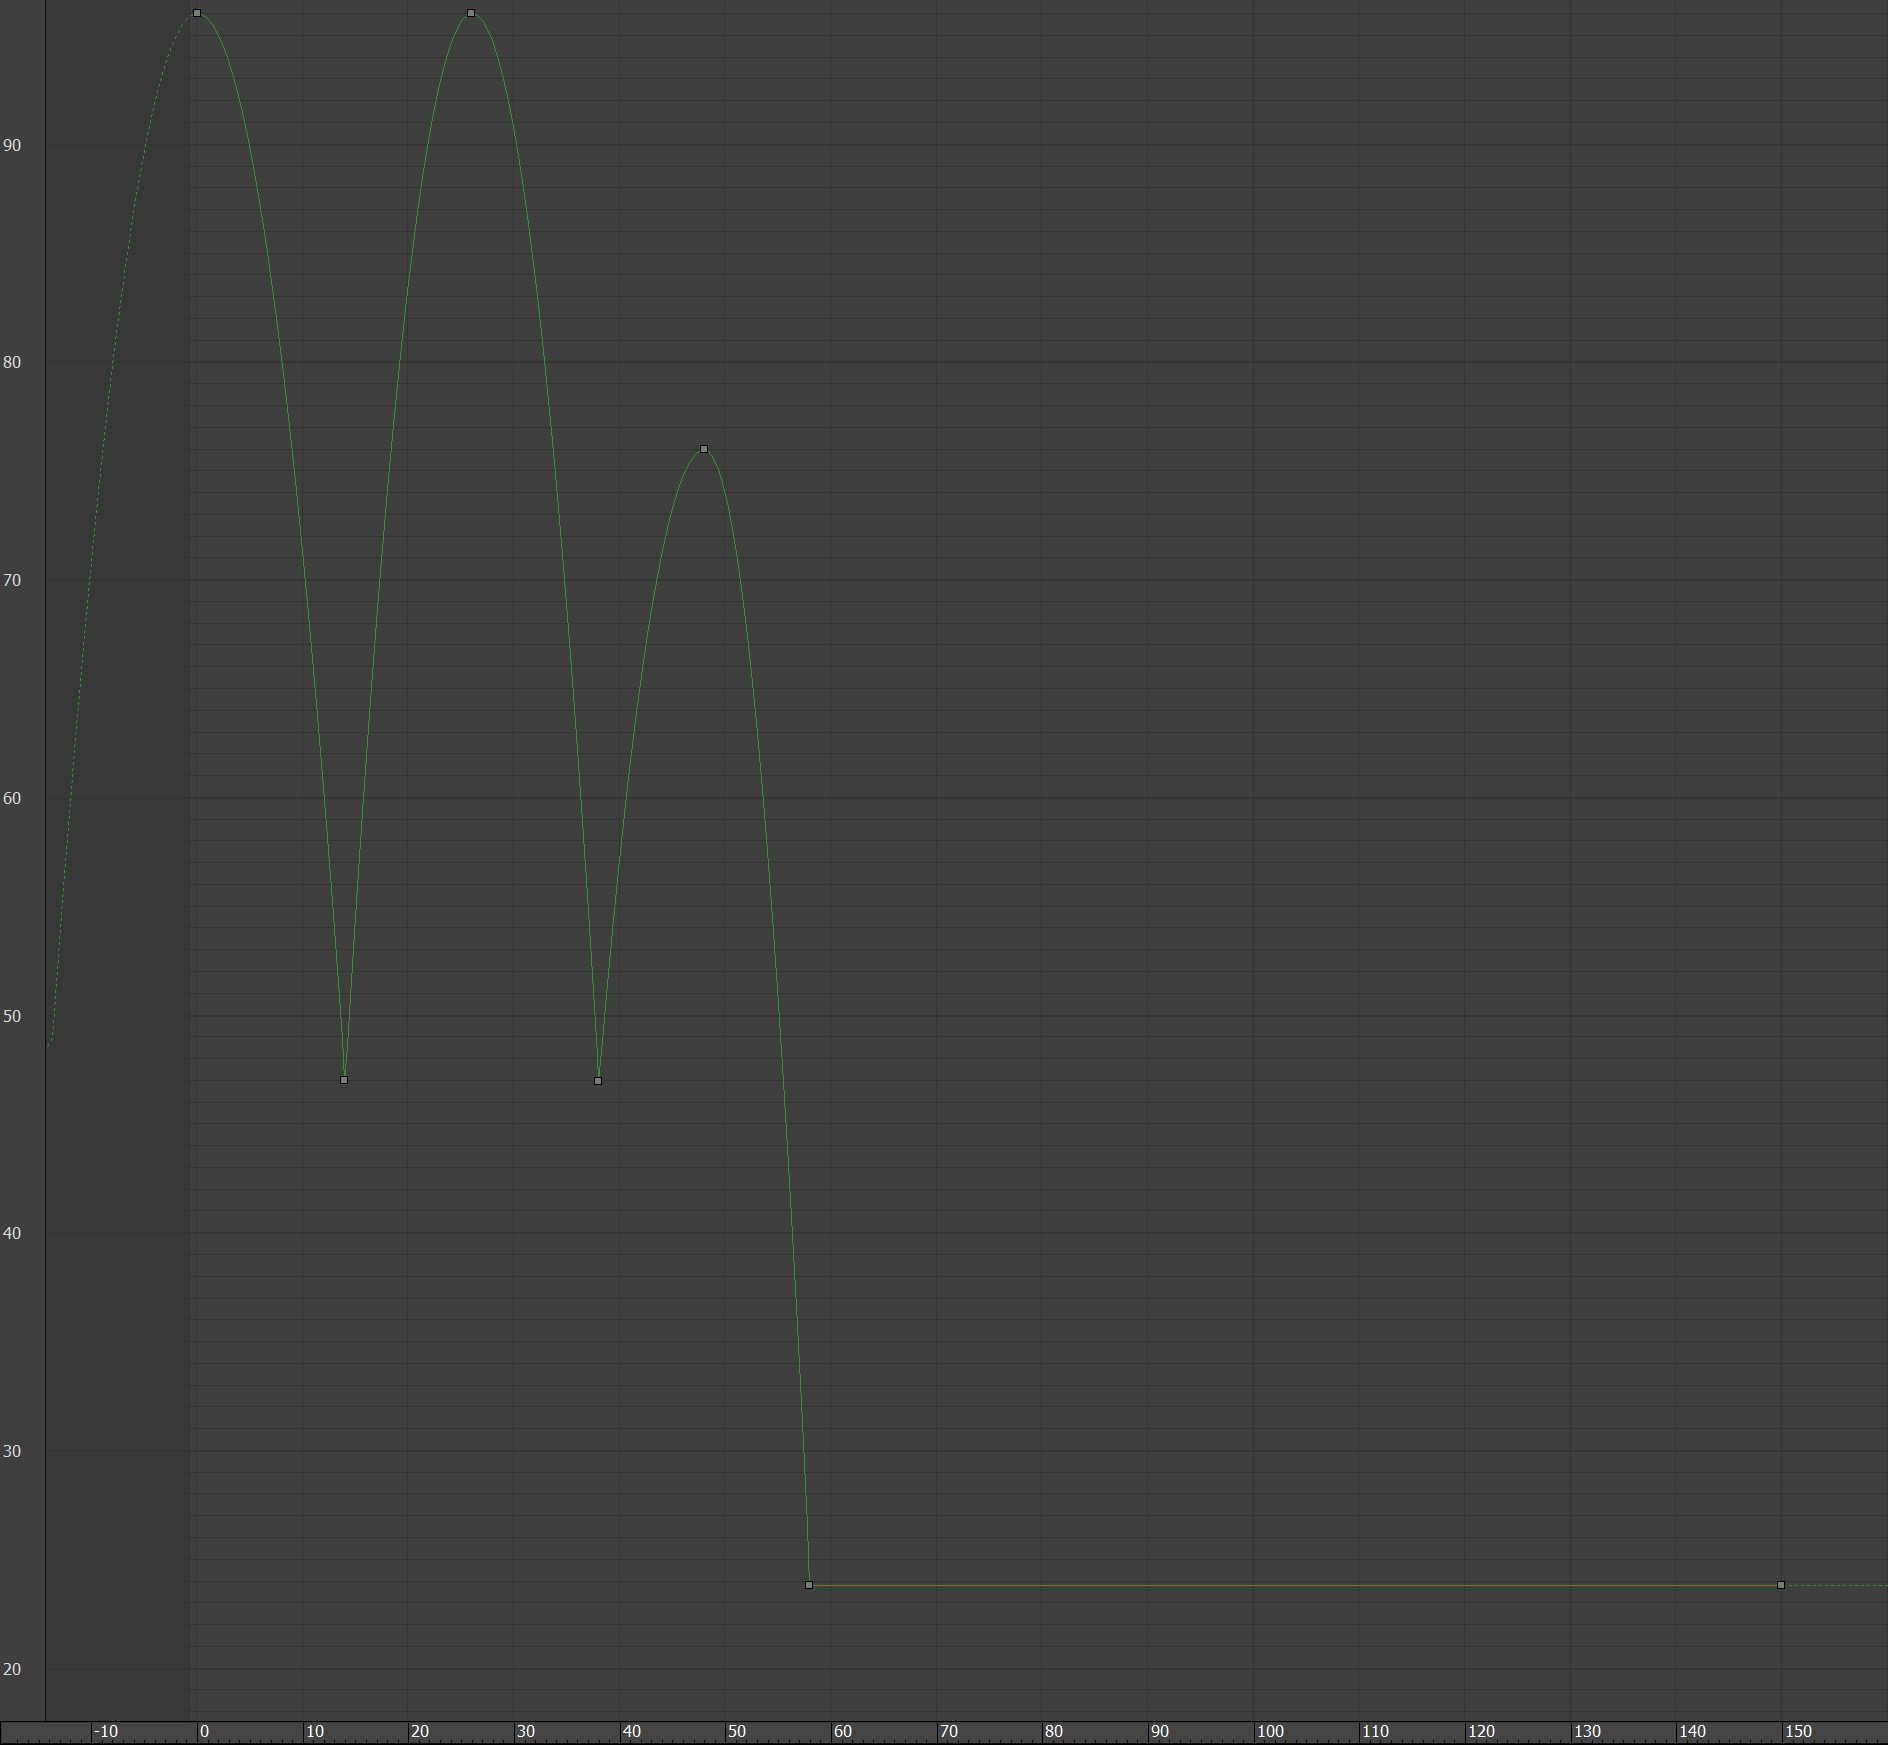
\includegraphics[width=\textwidth]{imagenes/curvas/PL/pelota/green.png}
   \caption{Curva que representa la posición en el eje Y de la pelota con respecto el tiempo.}
\end{figure}

Esta curva representa la posición en el eje Y de la pelota con respecto el tiempo. Realmente se ve reflejado en un cambio en el eje Z en coordenadas del mundo, pero a causa de usar los \textit{dummies}, este eje cambia. Sabiendo esto, se puede ver como la curva realiza una forma parabólica, simulando los efectos que tiene la gravedad sobre la pelota para acelerarla en la bajada y desacelerarla en la subida. Finalmente se queda parada sobre el trampolin y dicho estado se extiende hasta el instante 150, para que la animación inversa funcione.

\begin{figure}[H]
   \centering
   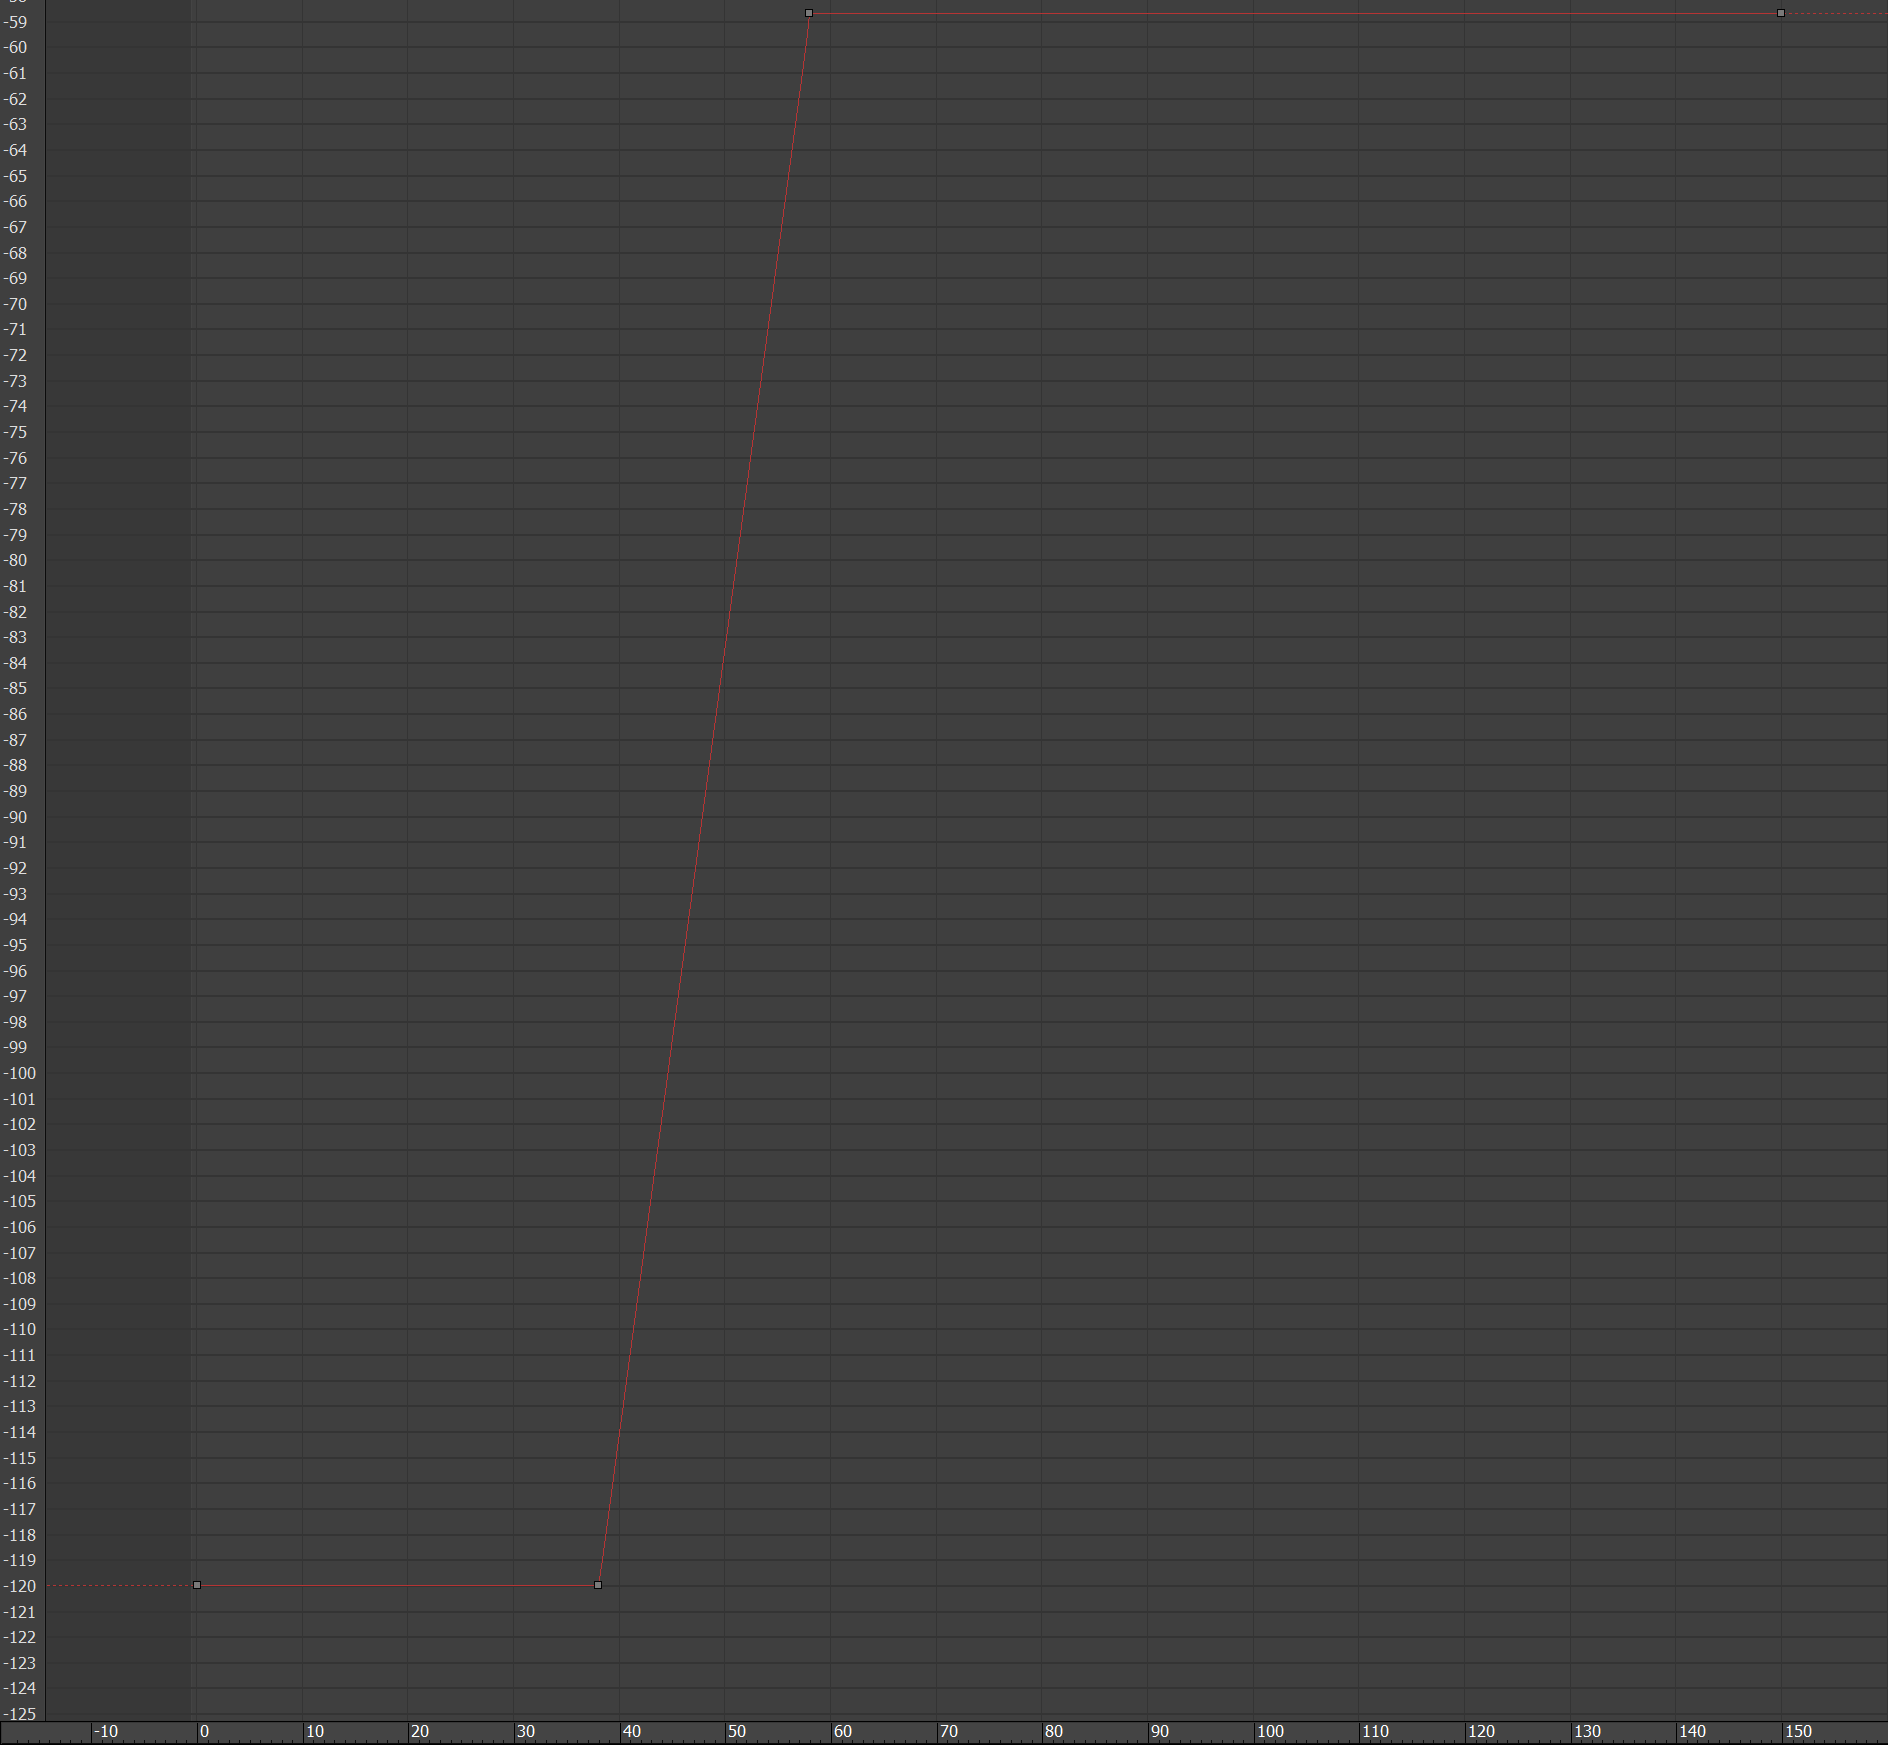
\includegraphics[width=\textwidth]{imagenes/curvas/PL/pelota/red.png}
   \caption{Curva que representa la posición en el eje X con respecto el tiempo.}
\end{figure}

% rescribir
Esta curva representa la posición en el eje X con respecto el tiempo, solo desde la posición de la base hasta en el momento que toca por primera vez el trampolin, ya que las siguientes animaciones las realiza el \textit{Dummy} correspondiente. He elegido una funcion lineal, ya que es la que me ha parecido mas realista de todas las opciones, dentro de lo que cabe. 


Los \textit{keyframes} para el \textit{Dummy} de la pelota de la izquierda son:

\begin{itemize}
    \item \textbf{Instante 0: }Se encuentra en su posición inicial, sin ninguna rotación para hacer que la trayectoria de la pelota sea correcta.
    \item \textbf{Instante 58: }Exactamente igual que el anterior \textit{keyframe}.
    \item \textbf{Instante 92: }El \textit{Dummy} se encuentra rotado hacia la izquierda, para animar el balanceo del balancin de manera correcta.
    \item \textbf{Instante 150: }Exactamente igual que el instante anterior, se hace para que la animación Ping-pong comienze al unísono con las demás.
\end{itemize}

Las curva de animación para el \textit{Dummy} son:

\begin{figure}[H]
    \centering
    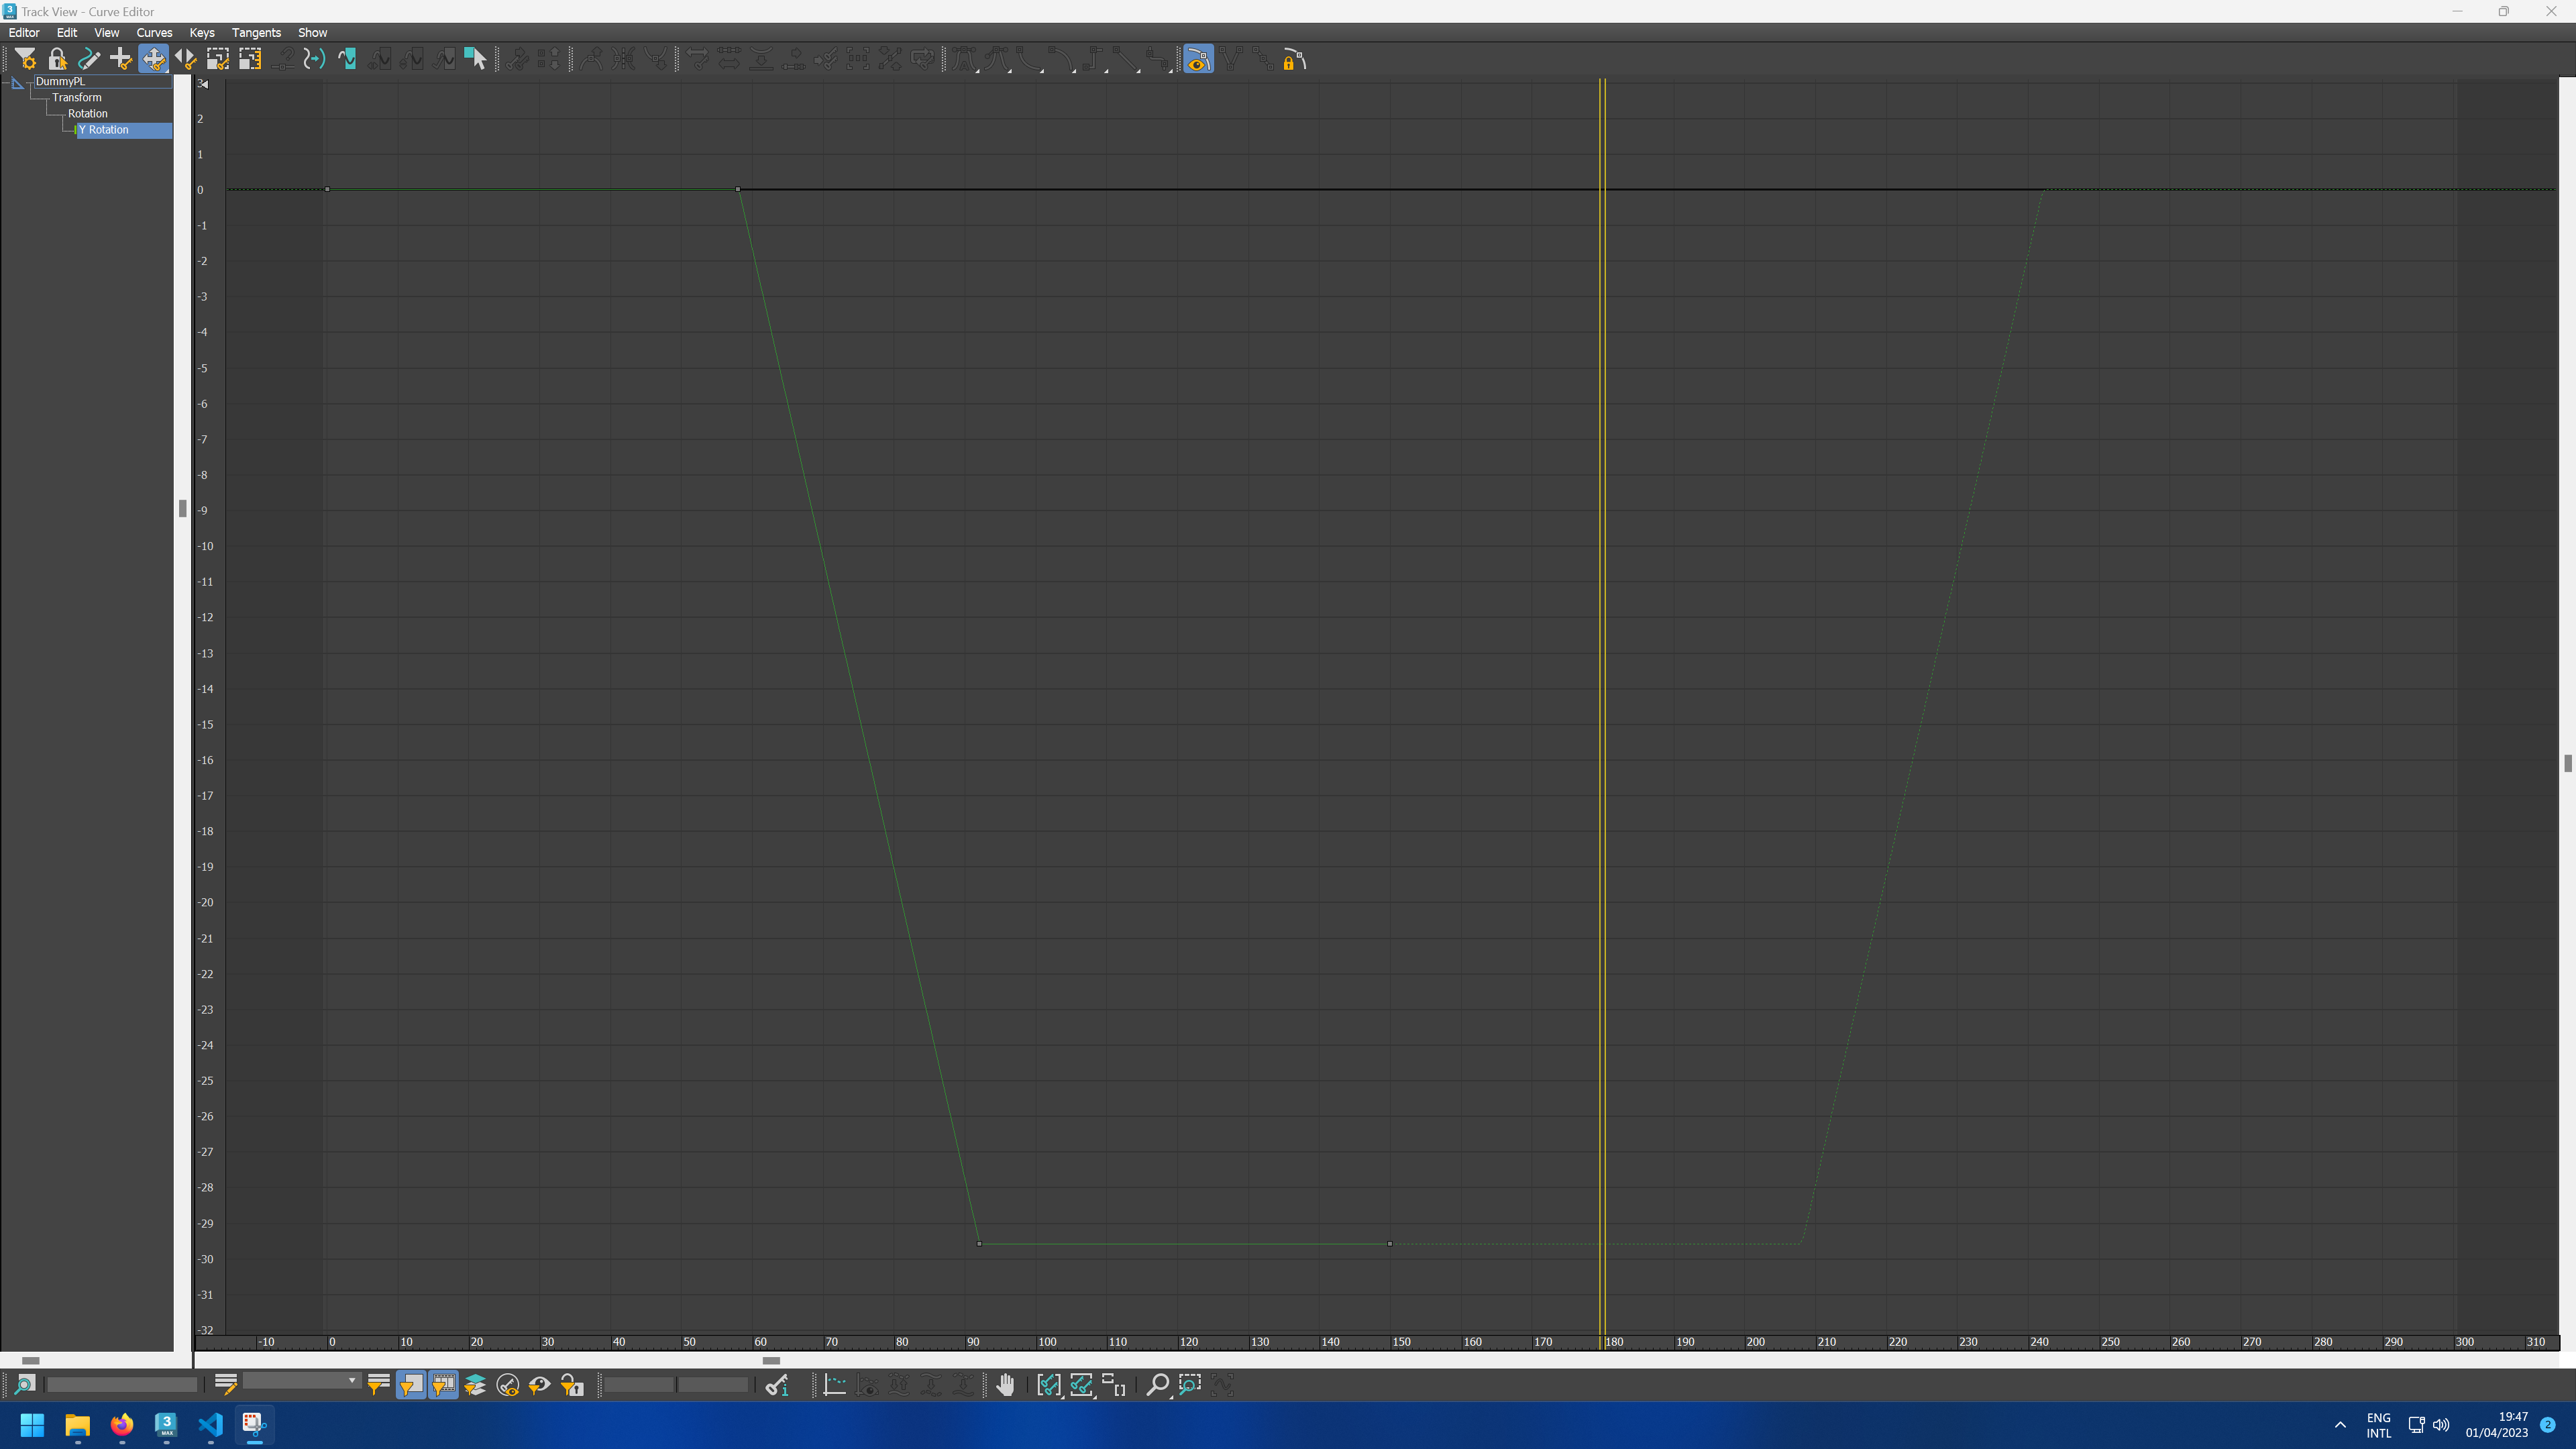
\includegraphics[width=\textwidth]{imagenes/curvas/PL/dummy/green.png}
    \caption{Curva que representa la rotación en el eje Y con respecto el tiempo.}
 \end{figure}

 % rescribir, muy repetido trampolin y pelota
Esta curva representa la rotación del \textit{dummy} con respecto al tiempo. La he animado de forma lineal porque, al seguir la animación del trampolin, esta debe seguirla tambien; es dedcir, como la energia potencial que tiene la pelota se le transfiere al trampolin, haciendo que el trampolin tenga la misma velocidad que la que tenia la pelota y no teniendo tiempo para acelerar.

\bigskip

Todo esto que he dicho es aplicable al trampolin, por lo que la explicacion correspondiente va a ser muy similar.

Y la trayectoria resultante es:

\begin{figure}[H]
    \centering
    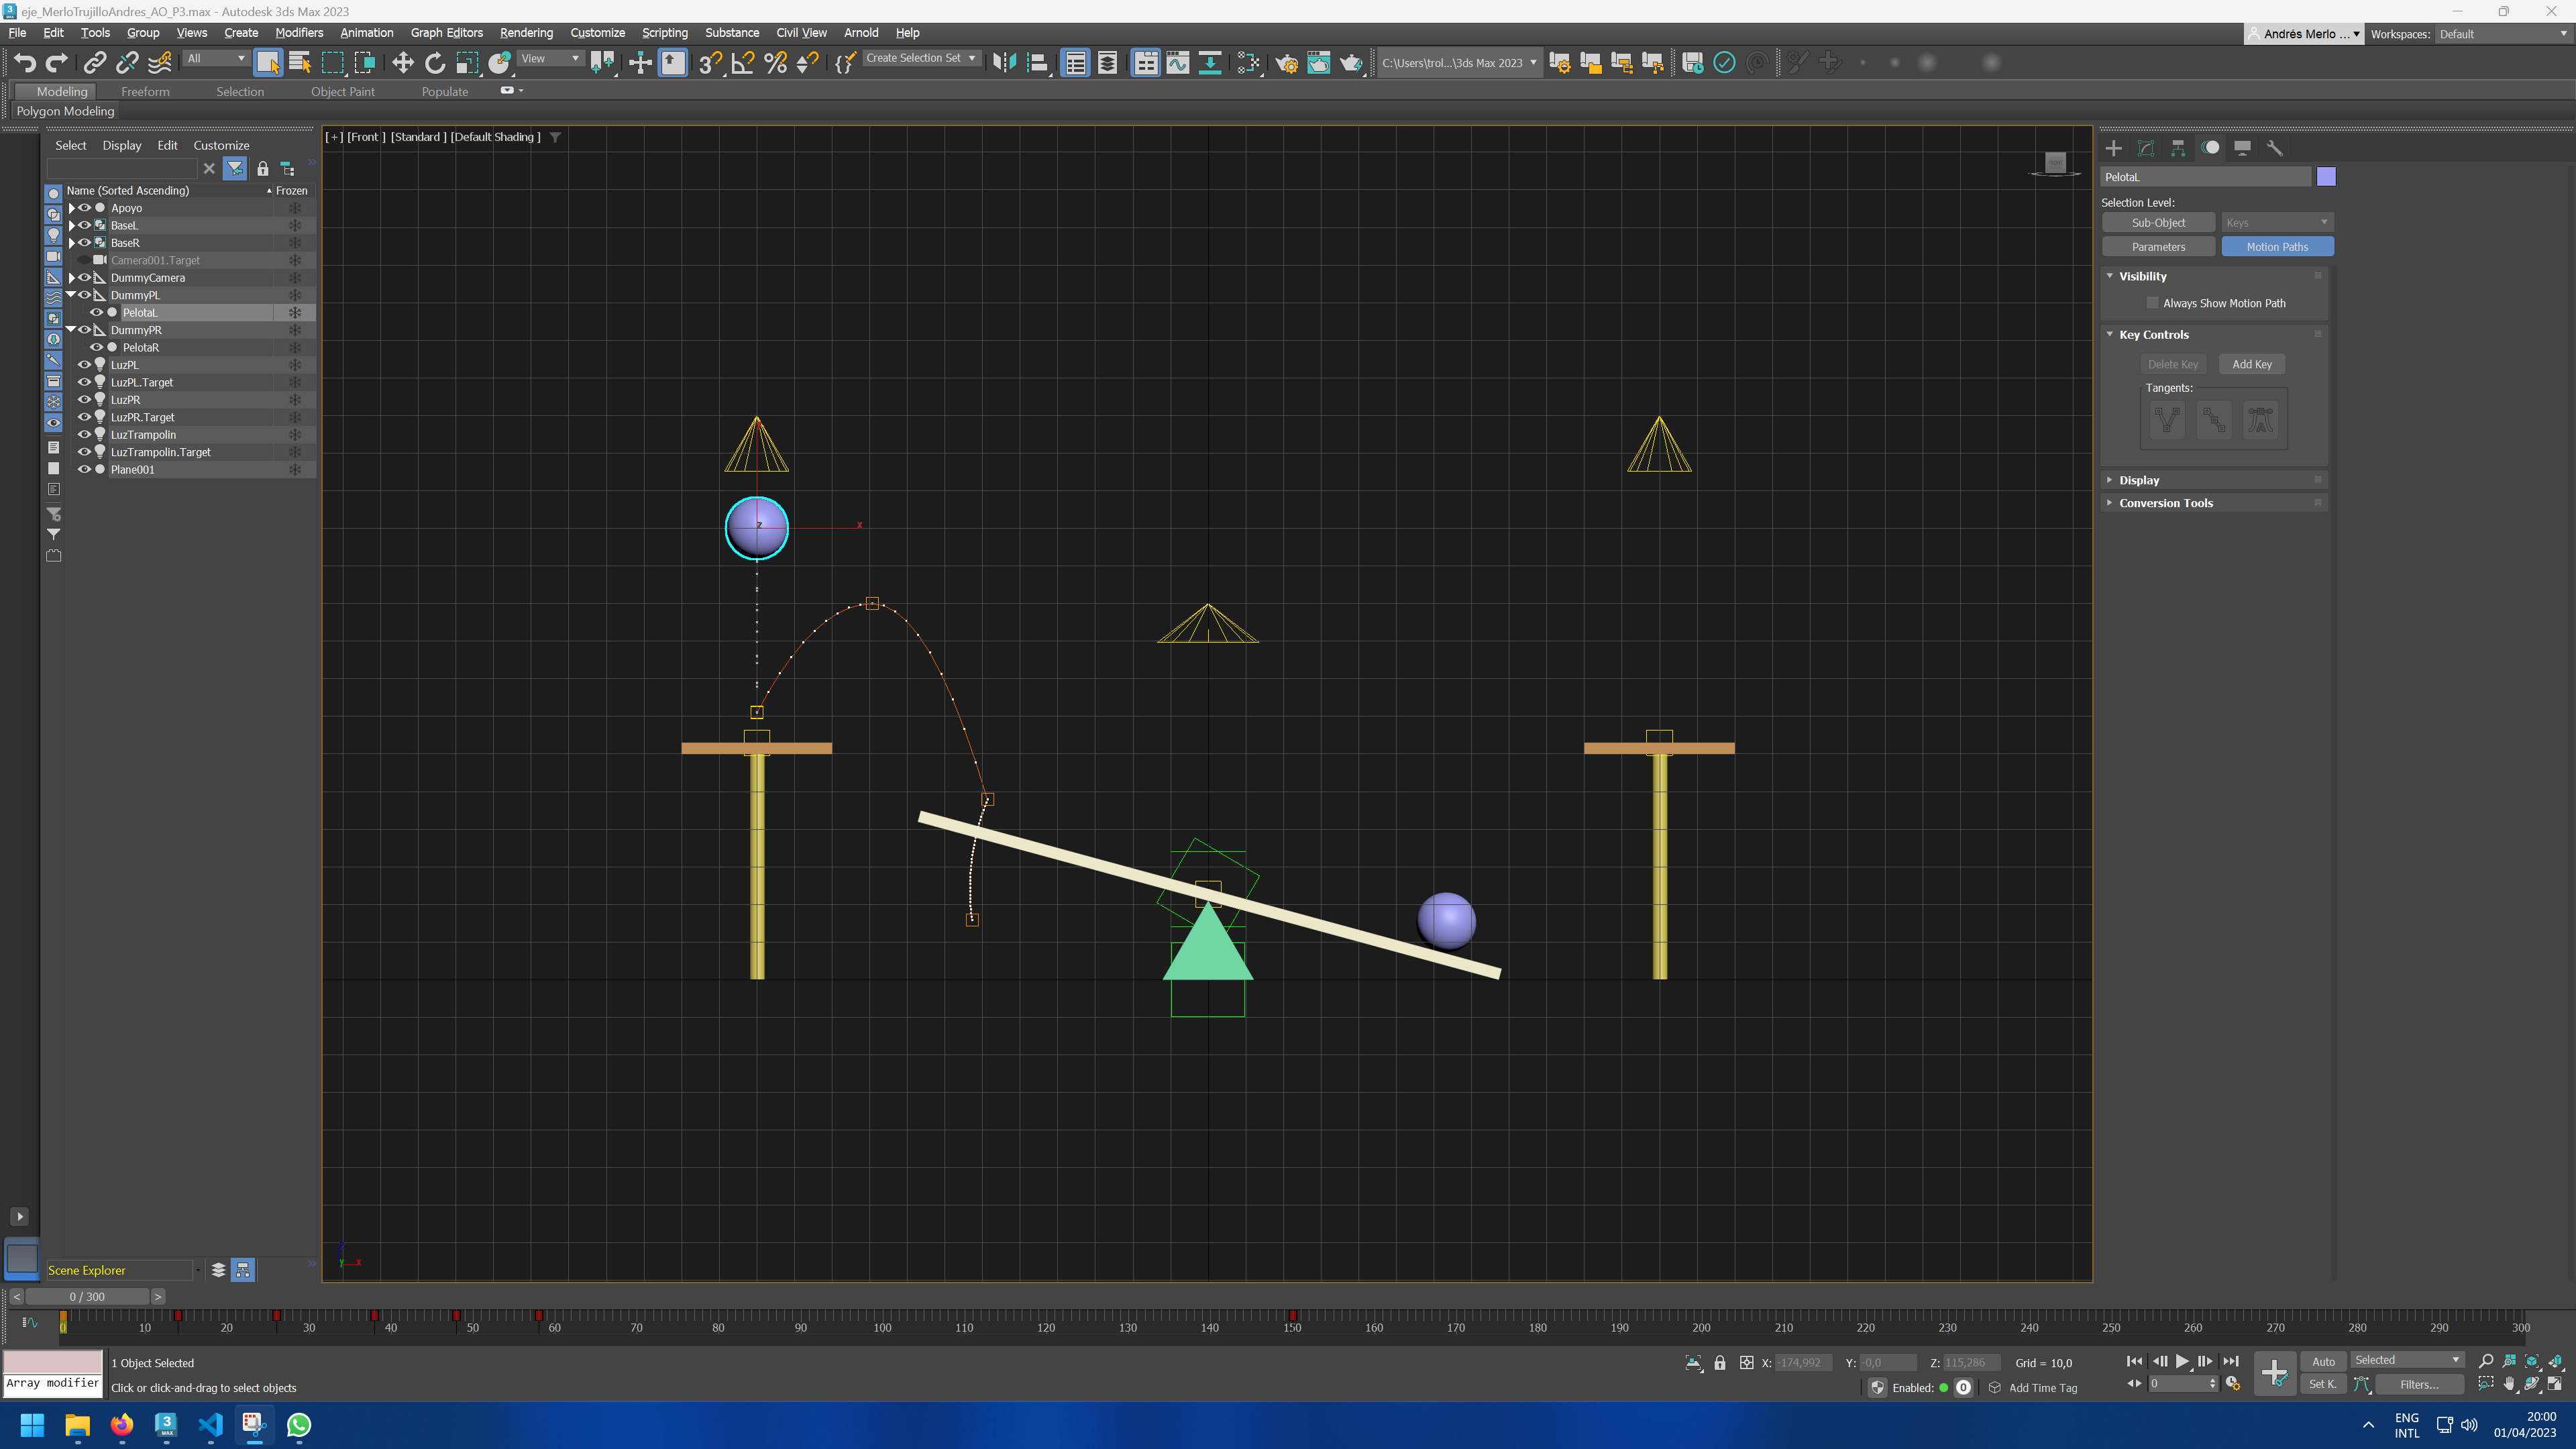
\includegraphics[width=\textwidth]{imagenes/animaciones/PL/pelota/motionpath.png}
    \caption{Trayectoria final que sigue la pelota.}
 \end{figure}


\subsection{Pelota de la derecha}
Los \textit{keyframes} de la pelota de la derecha son:

\begin{itemize}
    \item \textbf{Instante 0: }La pelota se encuentra sobre la superficie del trampolín. Este instante solo es una extensión para que la animación ping-pong funcione correctamente y al mismo tiempo.
    \item \textbf{Instante 92: }Exactamente igual que el instante anterior.
    \item \textbf{Instante 102: }La pelota se encuentra sobre el punto más alto de la trayectoria hacia la base.
    \item \textbf{Instante 112: }La pelota ha acabado de realizar la trayectoria y se encuentra sobre la superficie de la base.
    \item \textbf{Instante 124: }La pelota se encuentra en el aire porque ha realizado un rebote.
    \item \textbf{Instante 136: }Ahora la pelota ha caido al suelo.
    \item \textbf{Instante 150: }Finalmente, la pelota da otro rebote y se encuentra en el aire de nuevo.
\end{itemize}

Las curvas de animación es:

\begin{figure}[H]
    \centering
    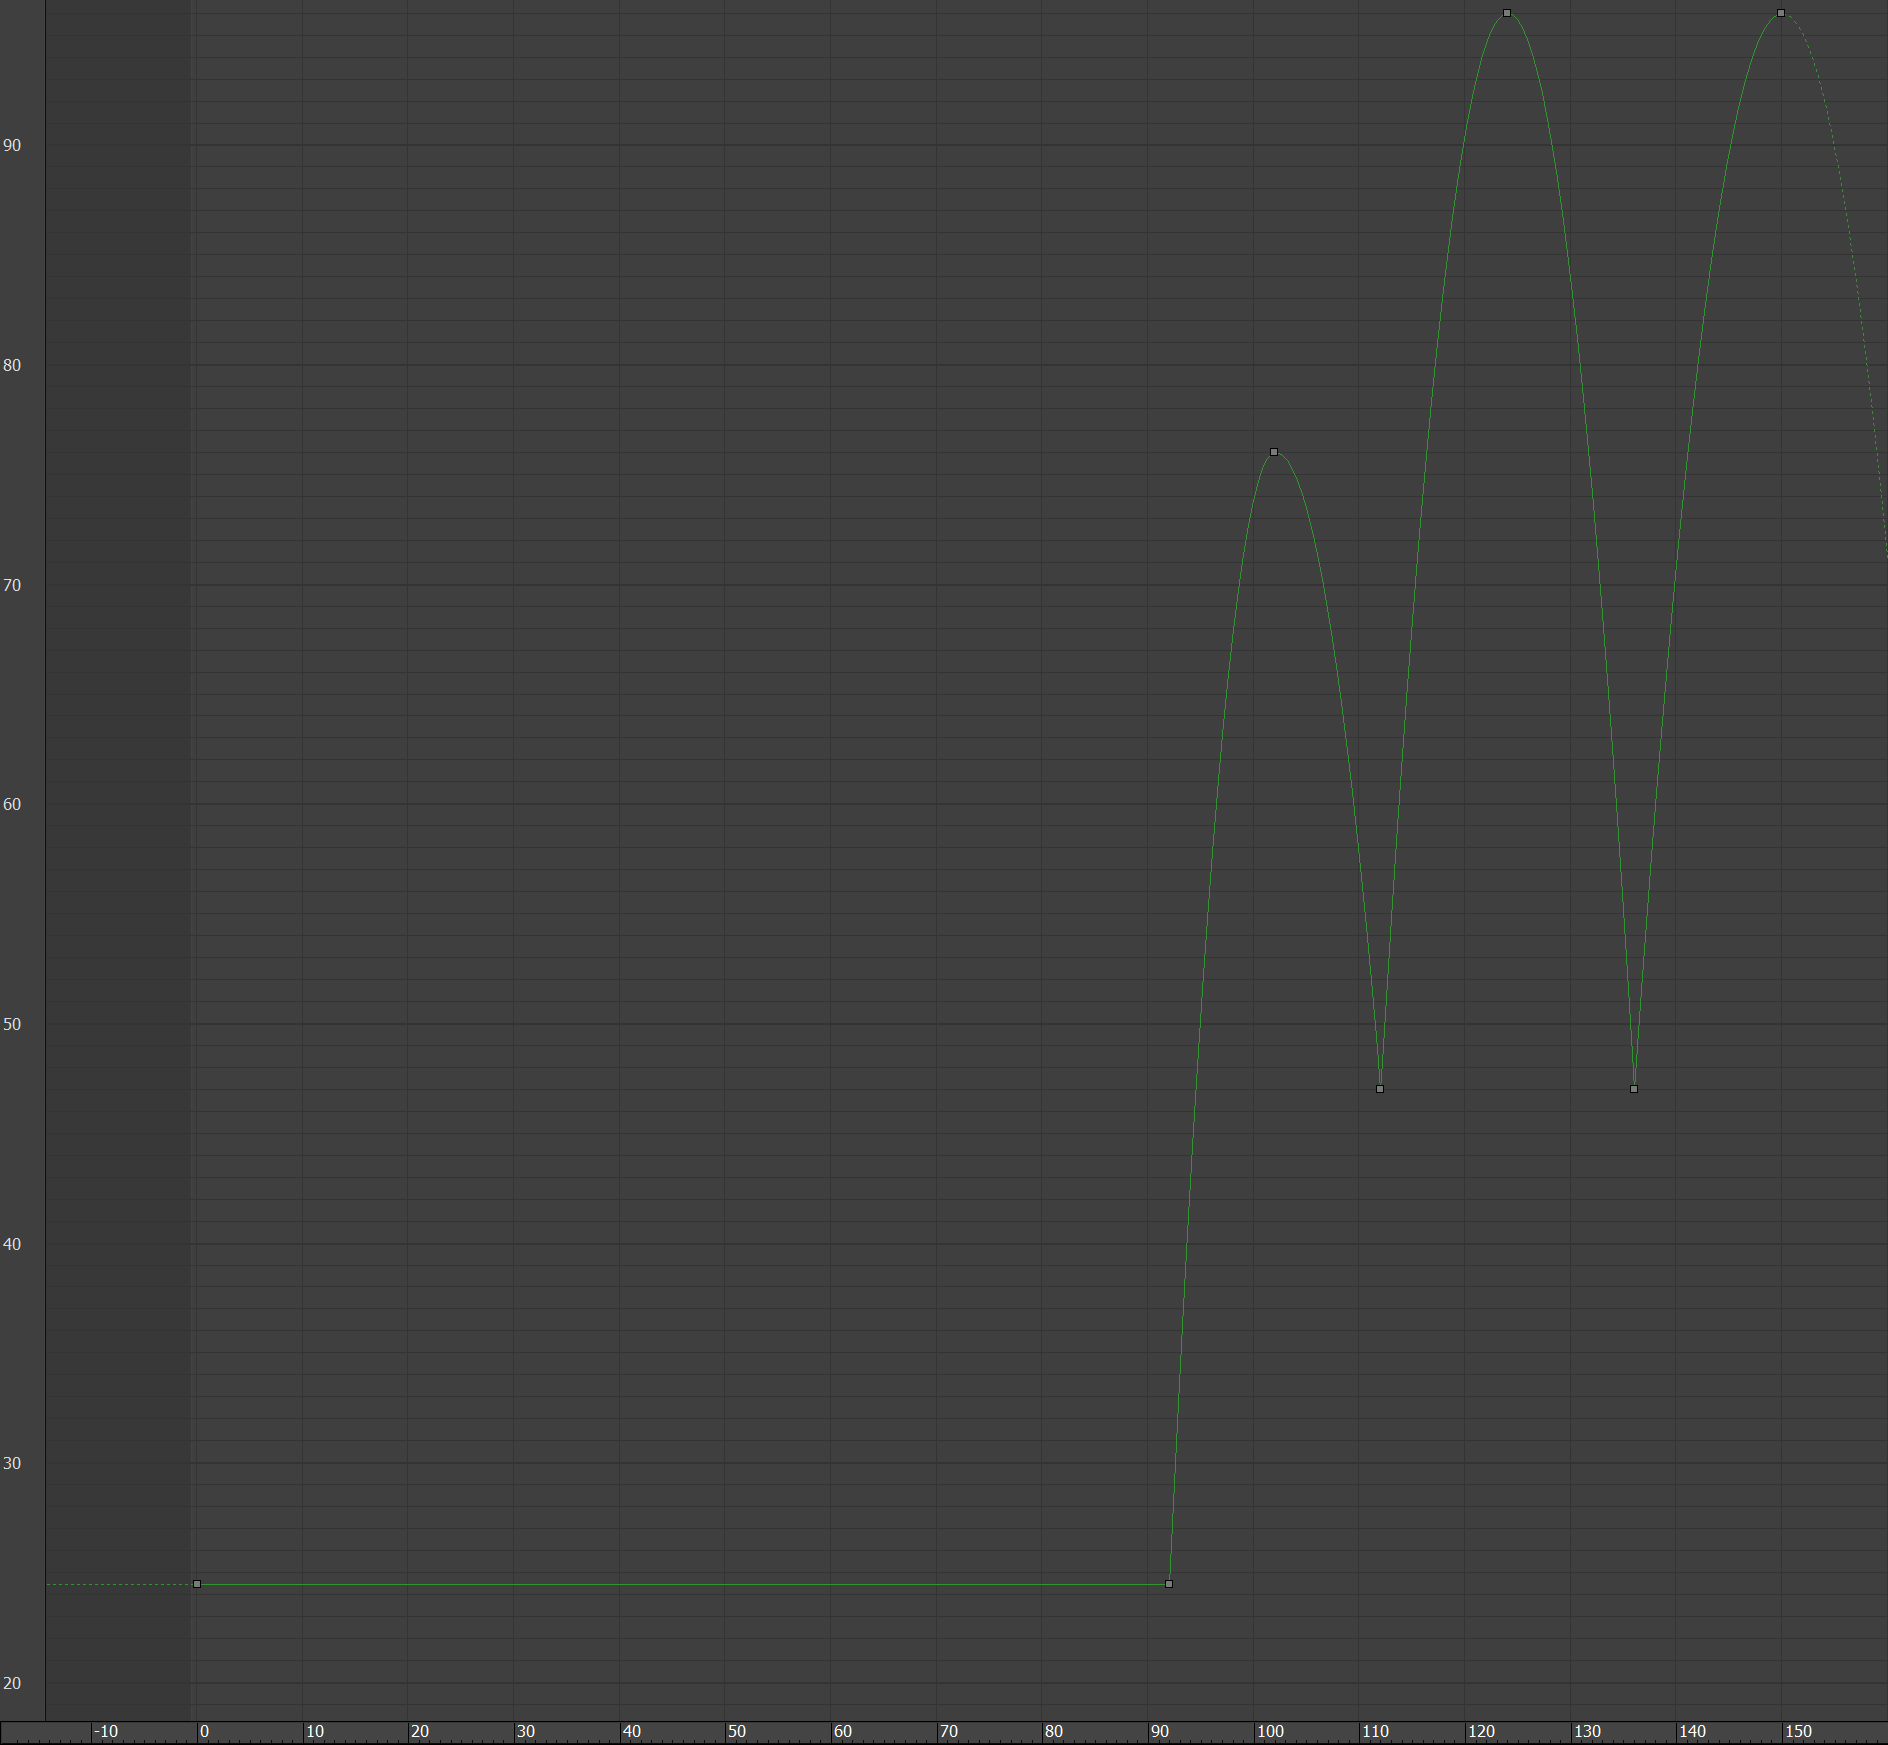
\includegraphics[width=\textwidth]{imagenes/curvas/PR/pelota/green.png}
    \caption{Curva que representa la posición en el eje Y con respecto el tiempo.}
 \end{figure}

 Al igual que con la pelota de la izquierda, debido al \textit{dummy} el eje Z pasa a ser el eje Y, pero en coordenadas del mundo sigue siendo el Z. Además, ocurre exactamente igual que en la pelota de la izquierda, se utilizan parábolas para simular los efectos de la gravedad sobre la pelota y que produzca un resultado natural, tanto en la trayectoria como en las subidas y caidas.

 \begin{figure}[H]
    \centering
    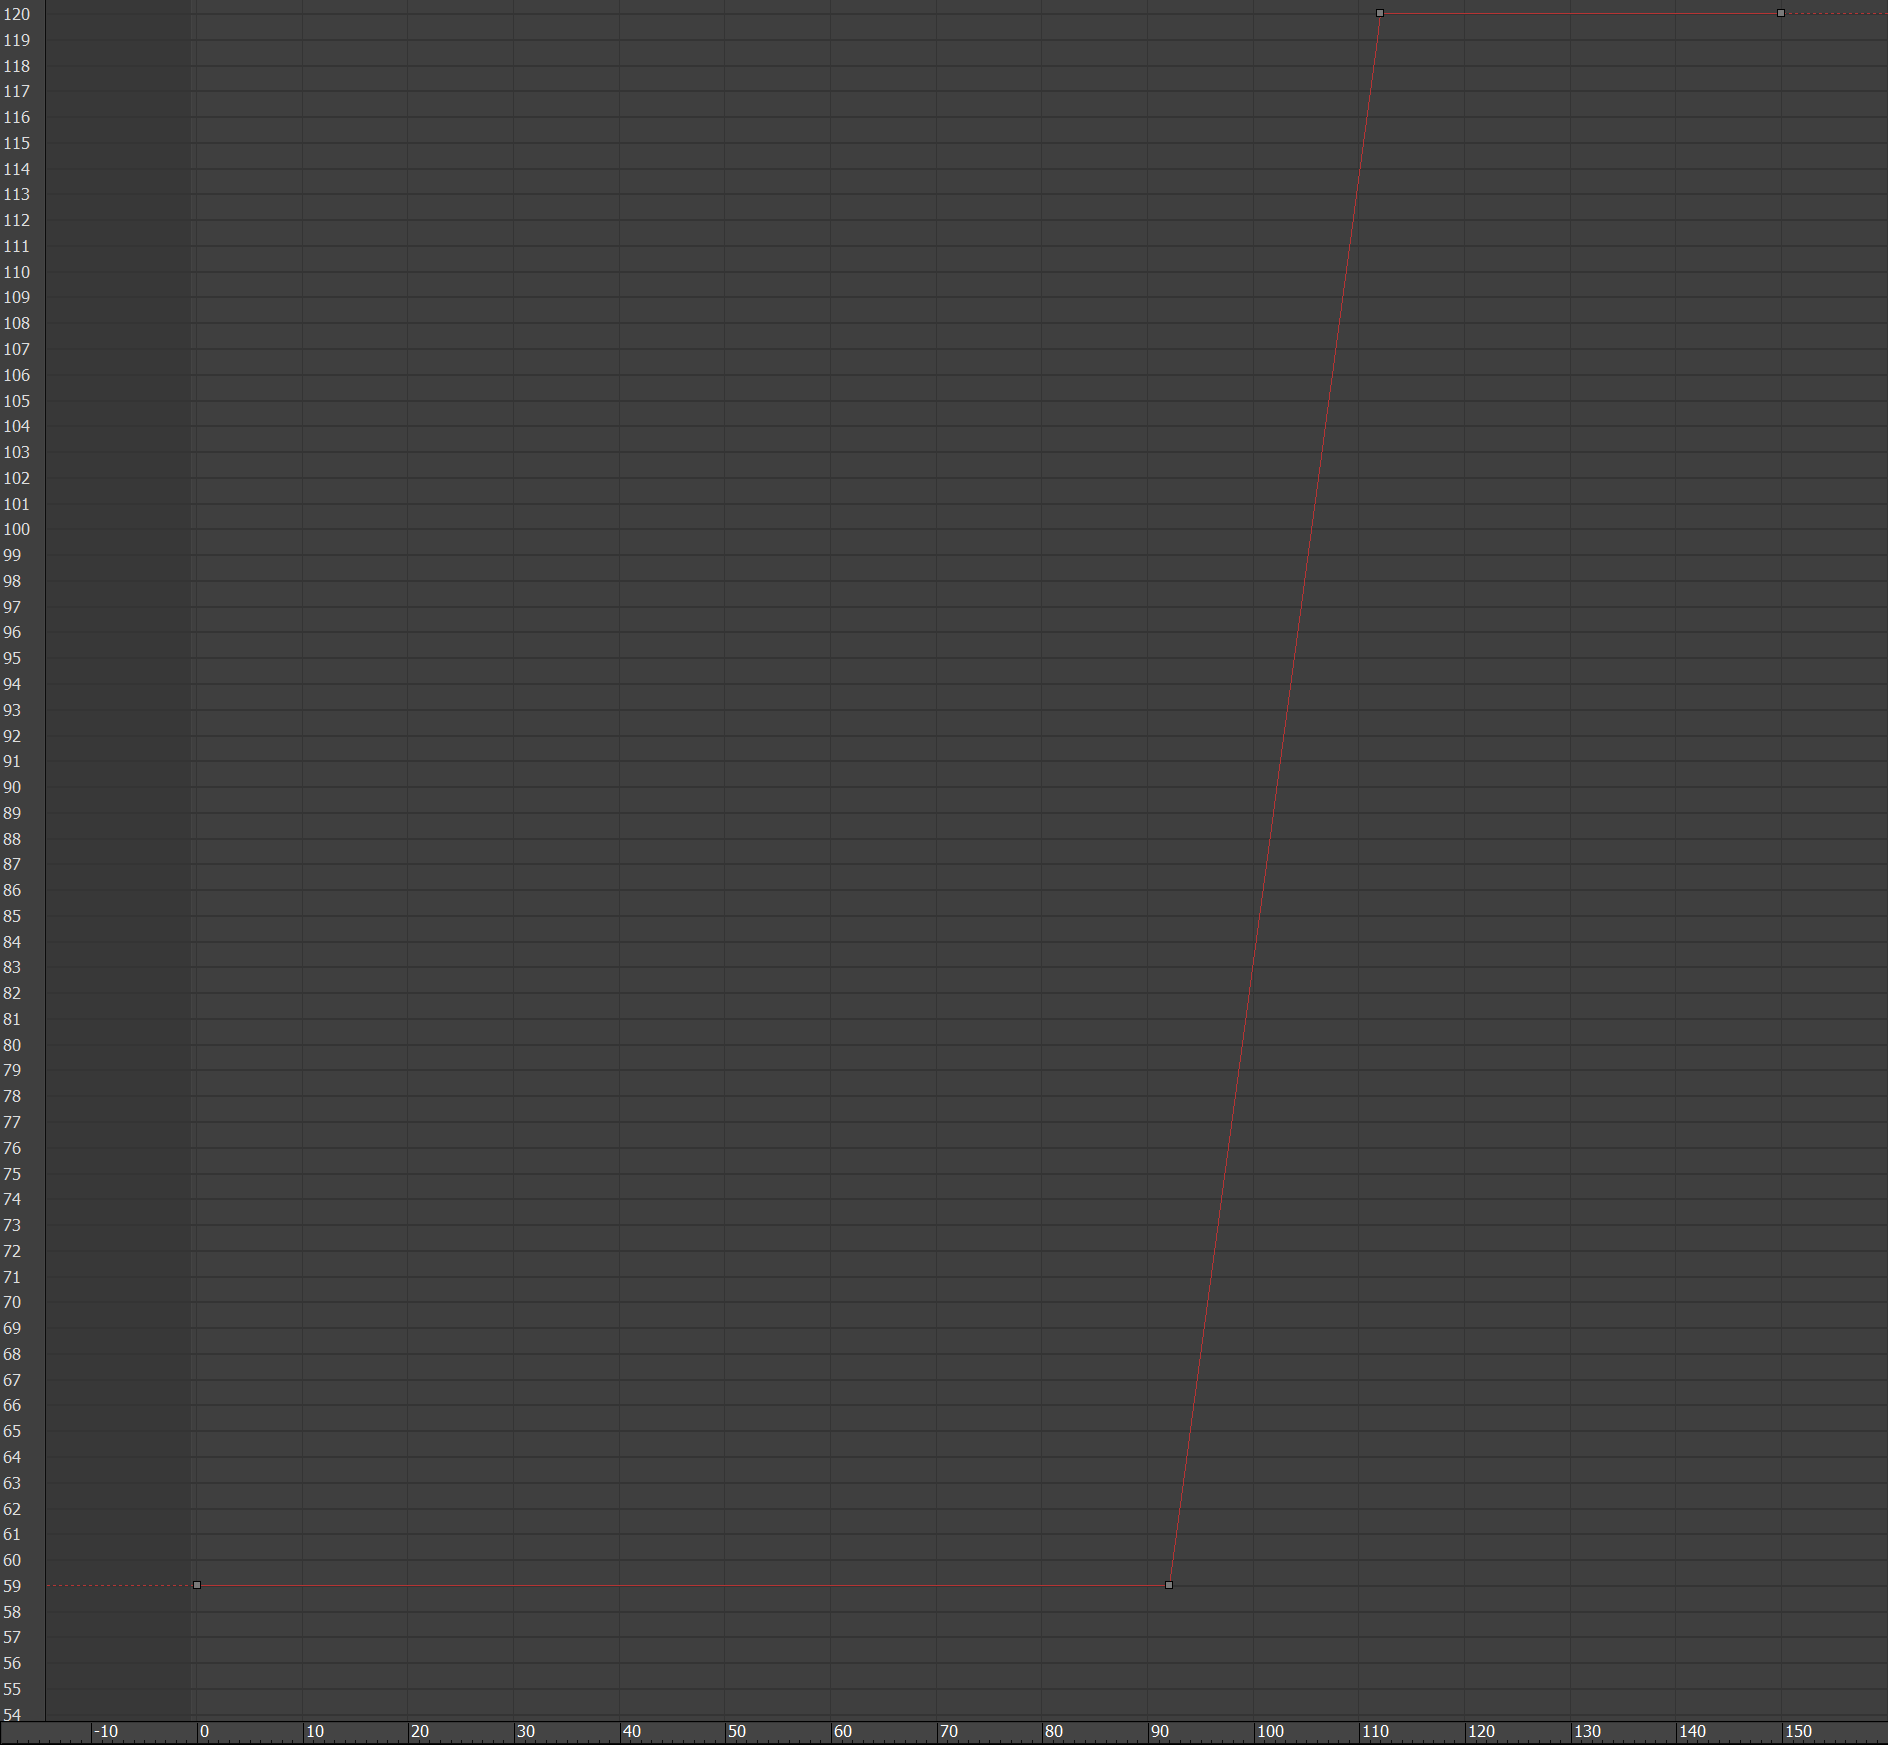
\includegraphics[width=\textwidth]{imagenes/curvas/PR/pelota/red.png}
    \caption{Curva que representa la posición en el eje X con respecto el tiempo.}
 \end{figure}

Esta curva representa la posición en el eje X con respecto al tiempo. Ocurre de manera similar que con la pelota izquierda, he utilizado una función lineal porque era la que me parecía más realista.


Mientras que los \textit{keyframes} para su \textit{Dummy} son:

\begin{itemize}
    \item \textbf{Instante 0: }El \textit{Dummy} se encuentra rotado para que la pelota se encuentre sobre el tramploin. Al igual que con la pelota, se debe hacer para que la animacion inversa se haga al mismo tiempo.
    \item \textbf{Instante 58: }No ha habido cambios en la animación, es igual que el instante anterior.
    \item \textbf{Instante 92: }Ahora el \textit{Dummy} se encuentra rotado en la posición original; es decir, sin ninguna rotación aplicada para que la trayectoria de la pelota sea correcta.
    \item \textbf{Instante 150: }Ningún cambio realizado, solo es para que la animación inversa comience a la misma vez.
\end{itemize}

La curva de animacion para el \textit{Dummy} es:

\begin{figure}[H]
    \centering
    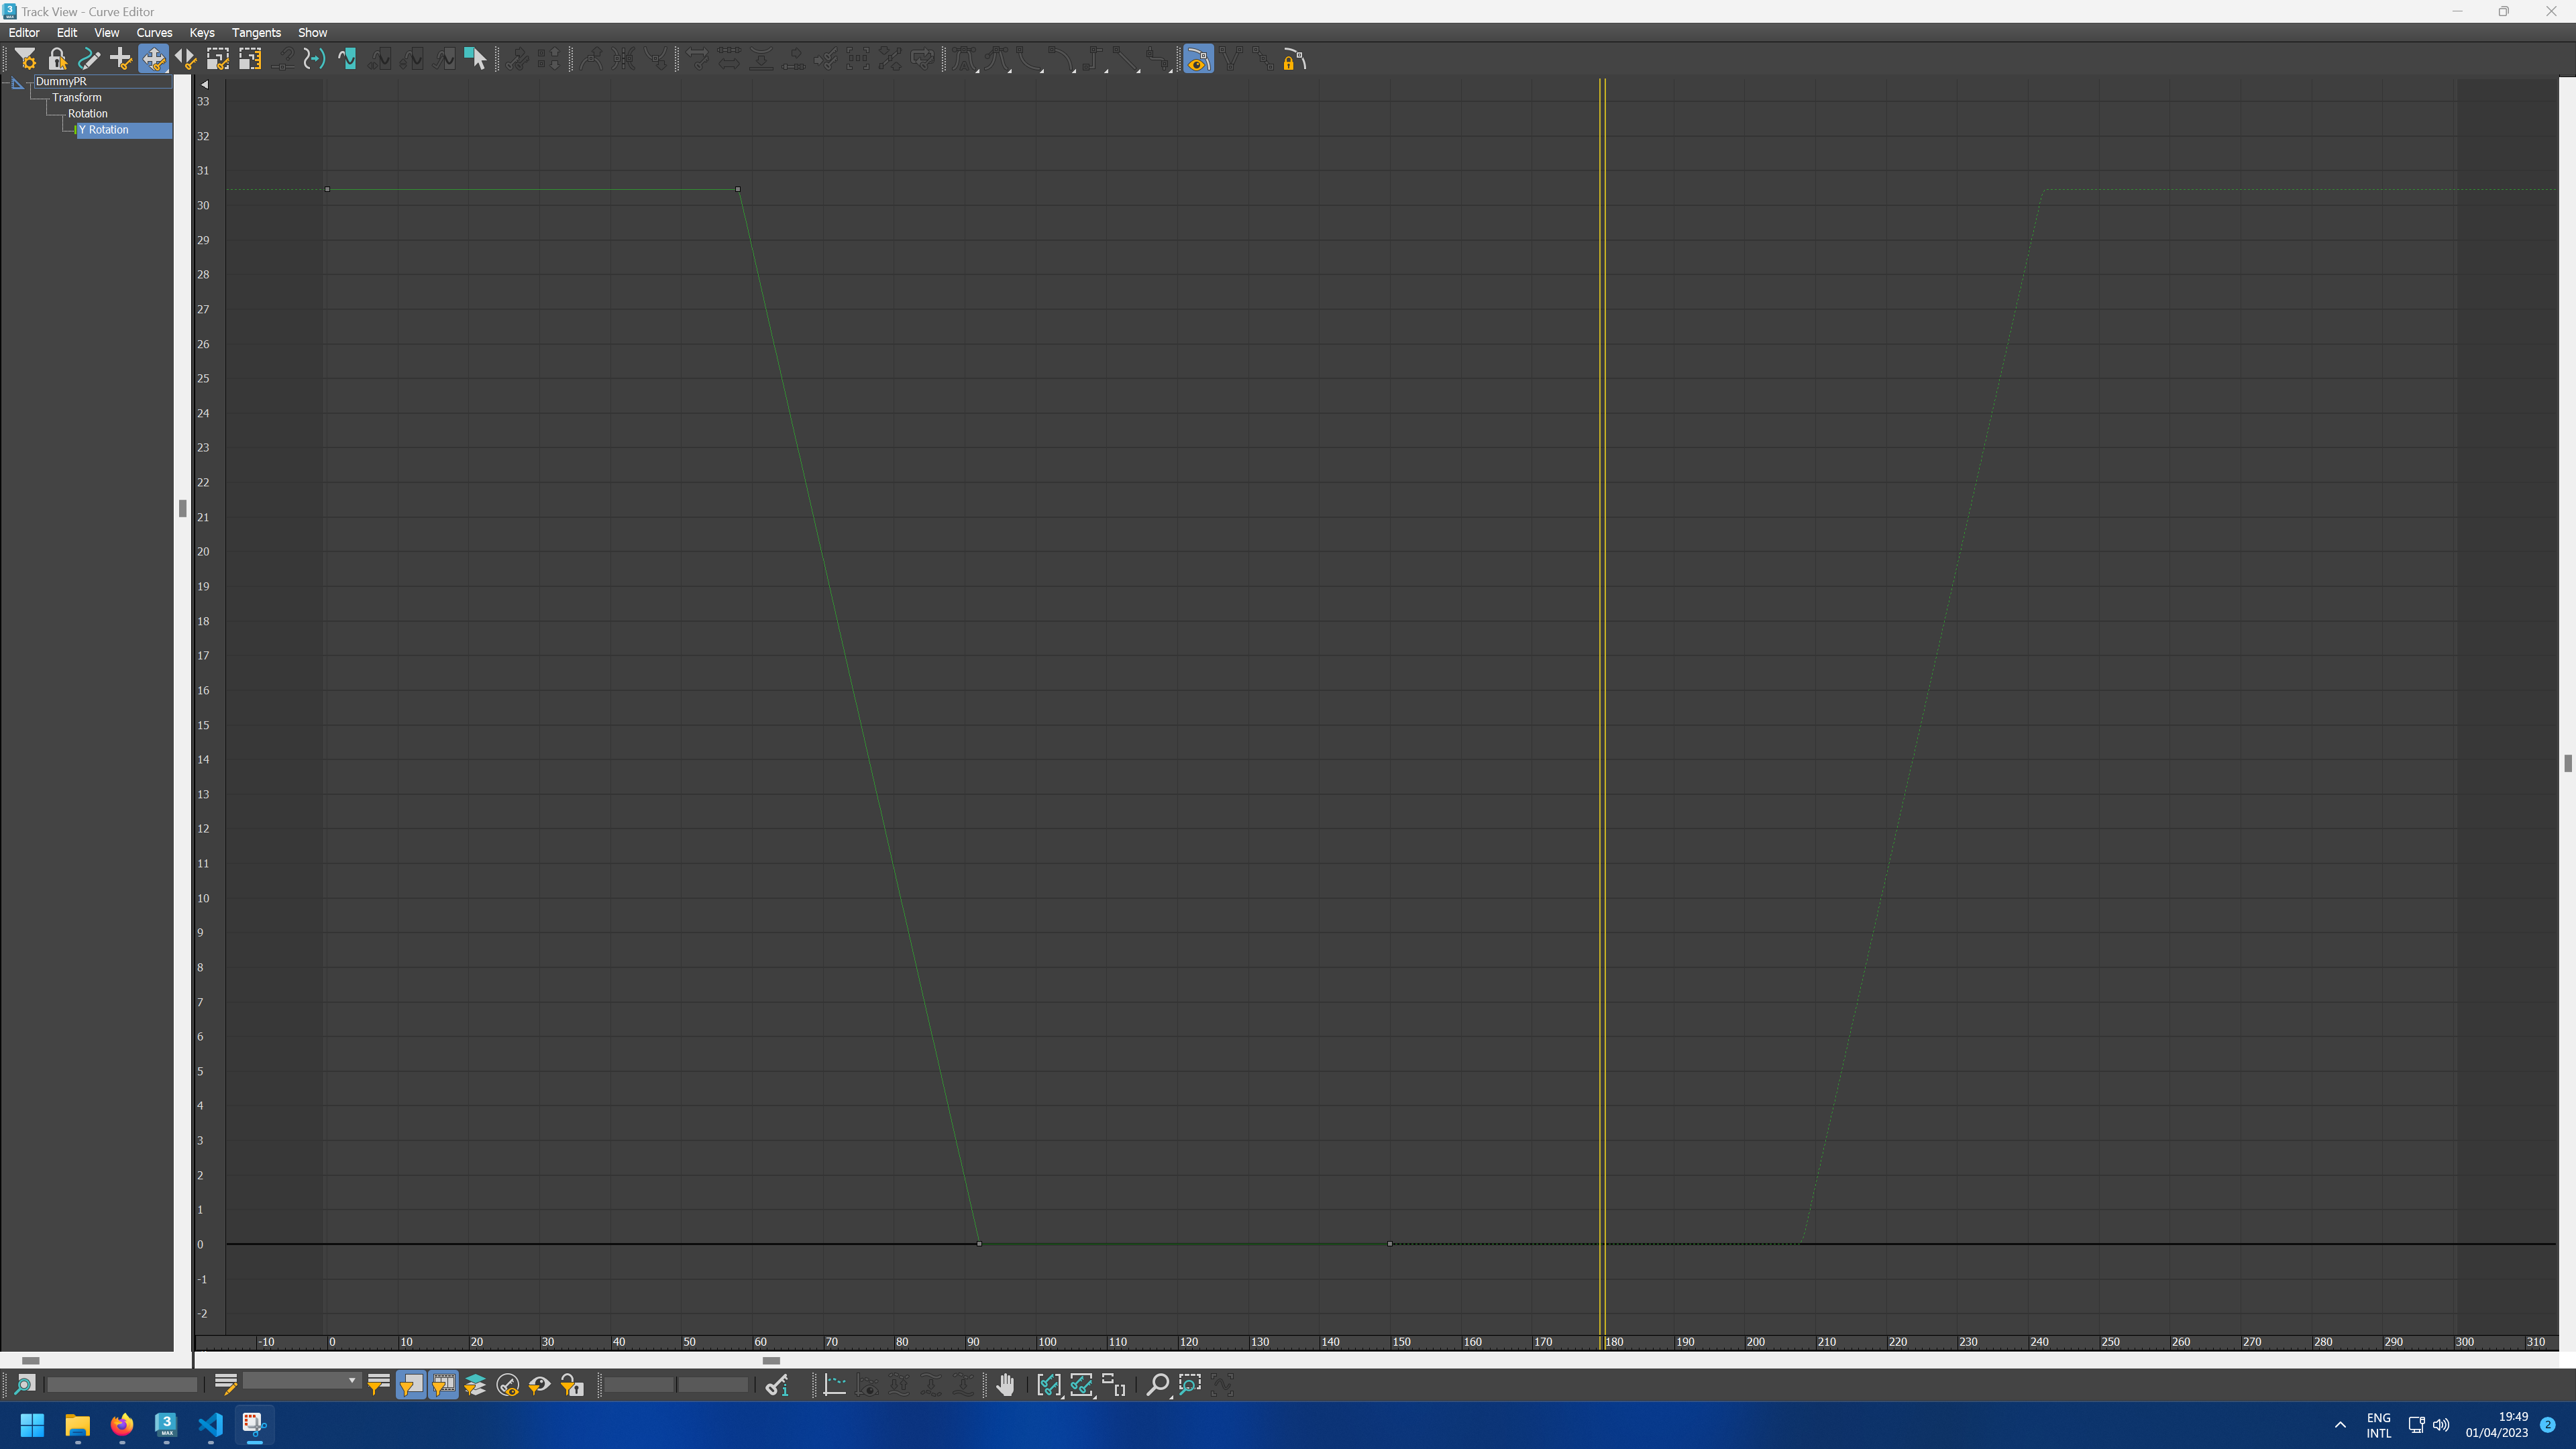
\includegraphics[width=\textwidth]{imagenes/curvas/PR/dummy/green.png}
    \caption{Curva que representa la rotación en el eje Y con respecto el tiempo.}
 \end{figure}

De nuevo, ocurre de manera similar que con el \textit{Dummy} de la otra pelota. La curva es lineal, ya que la pelota le transfiere al trampolín toda la energía potencial que tenía, haciendo que no tenga tiempo de acelerar y se ponga a la velocidad máxima directamente.

Y la trayectoria resultante es:

\begin{figure}[H]
    \centering
    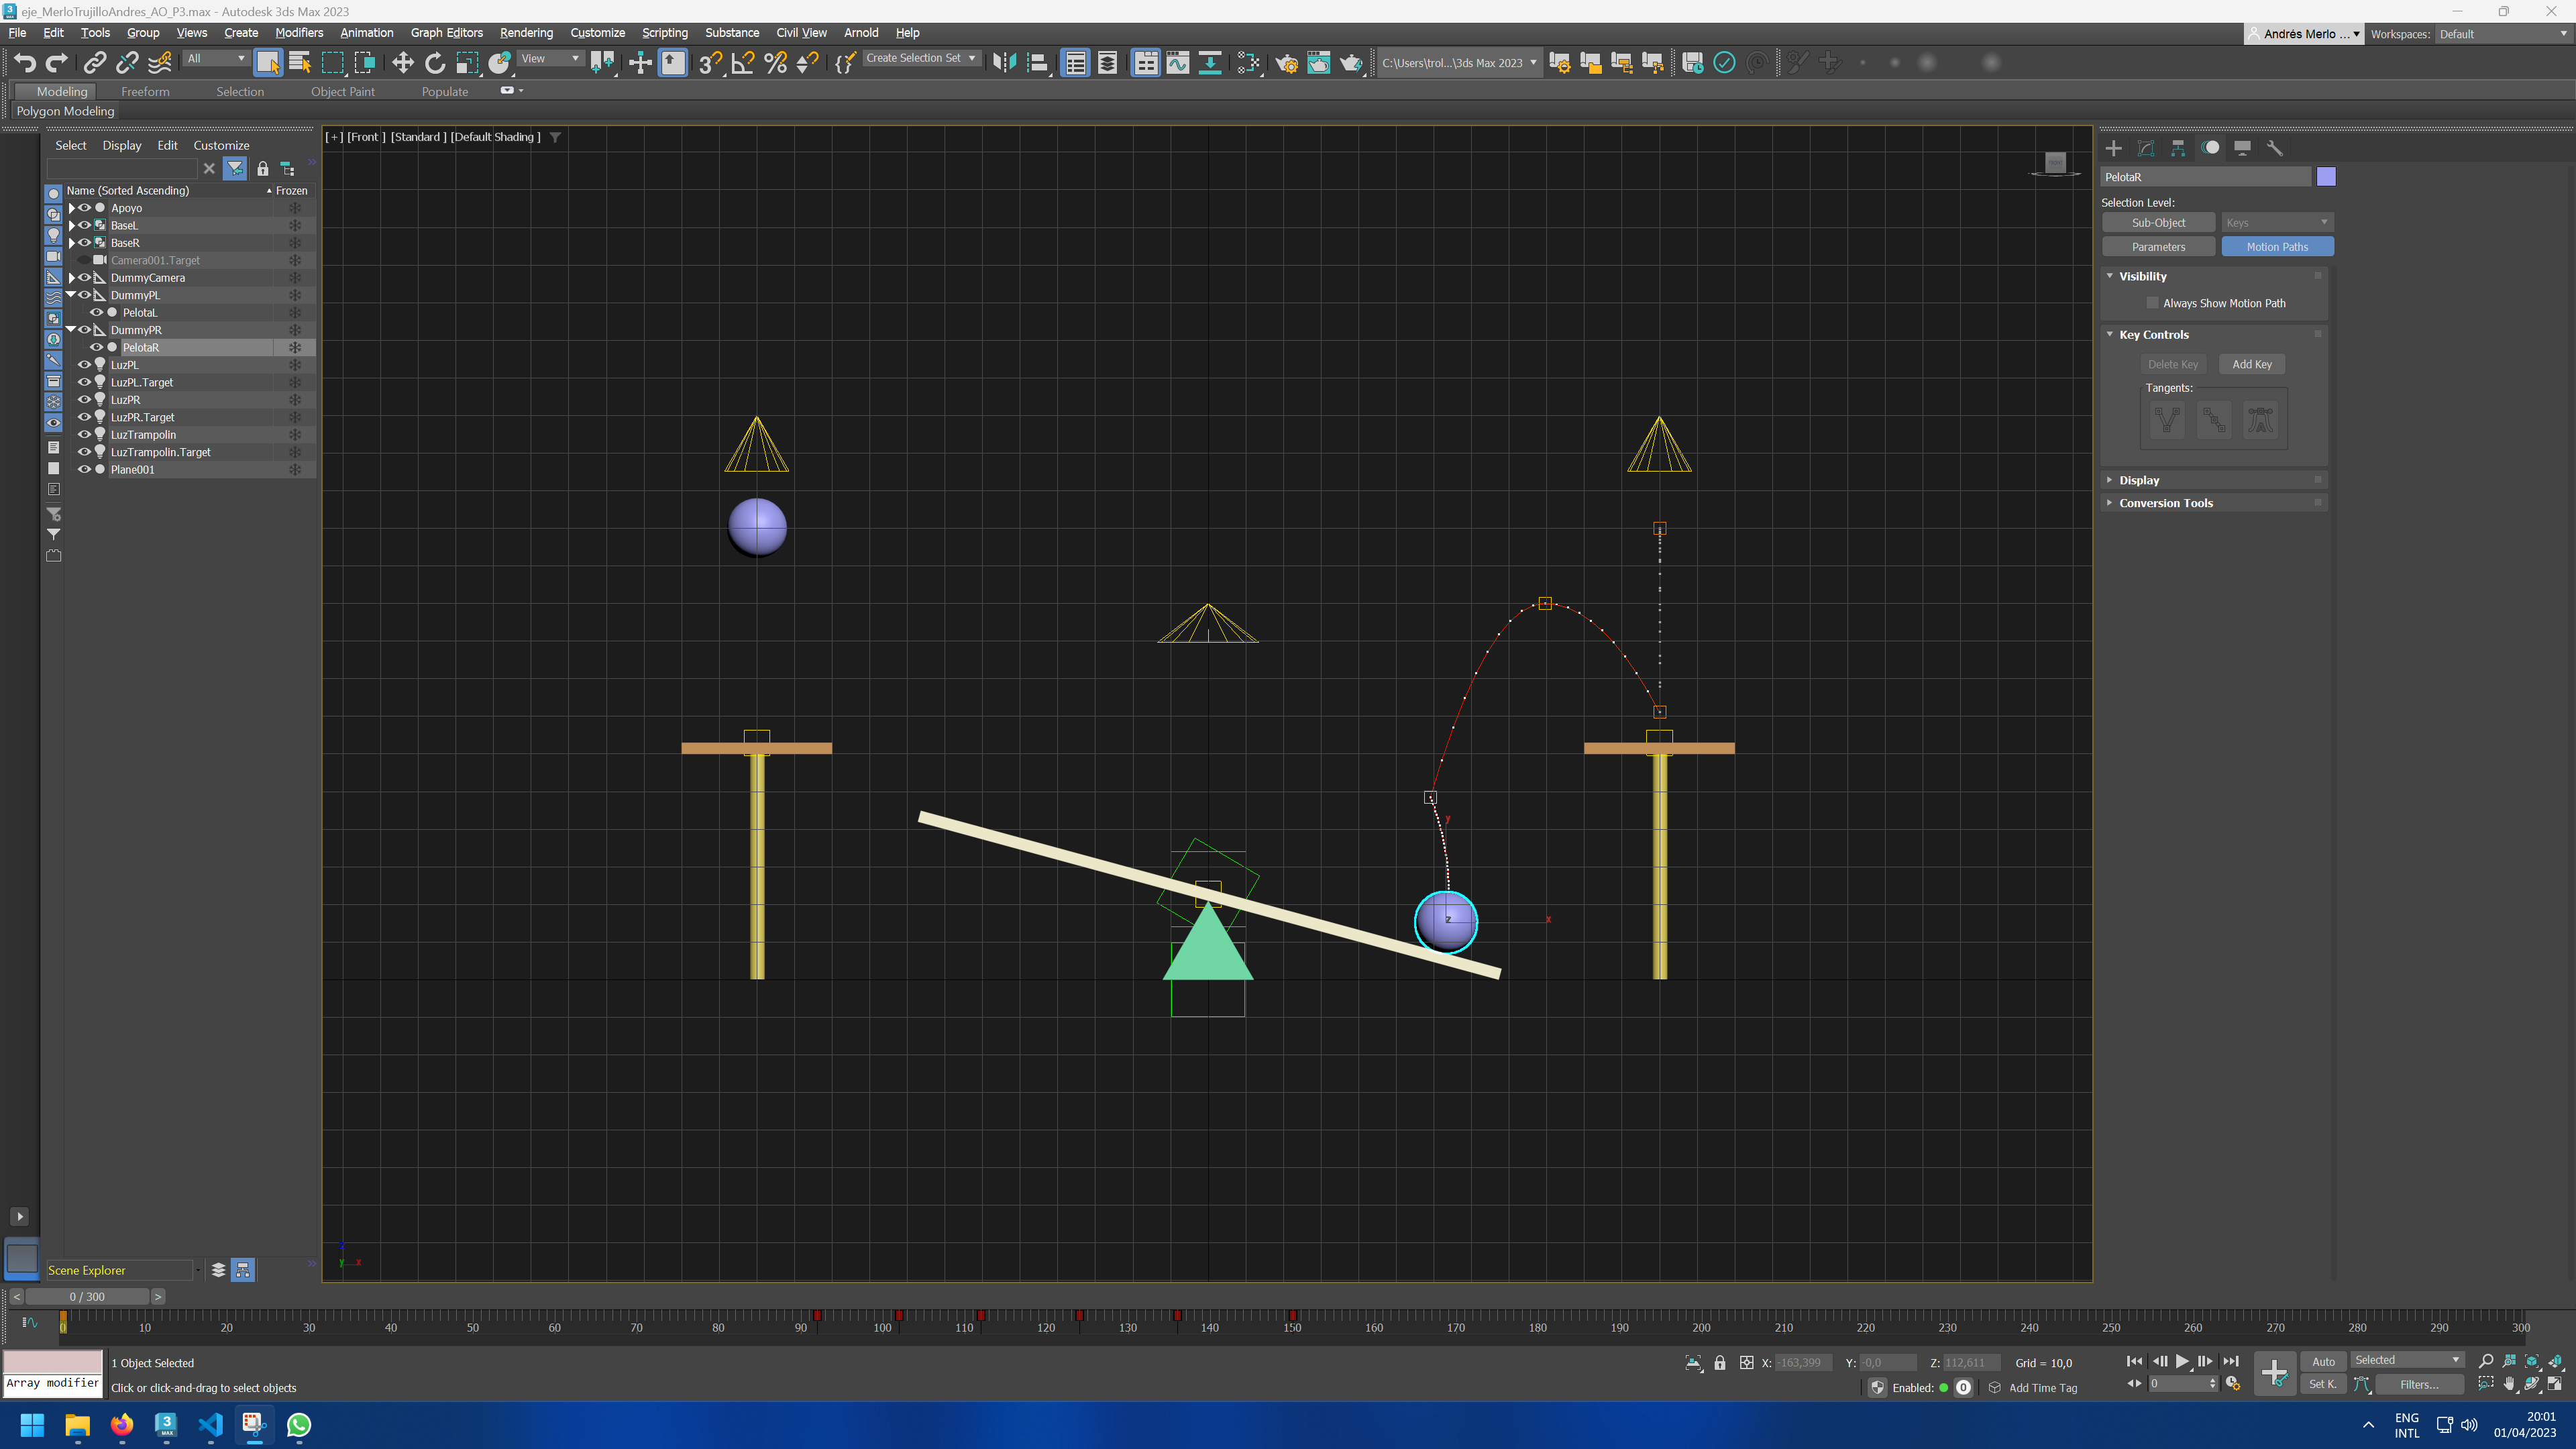
\includegraphics[width=\textwidth]{imagenes/animaciones/PR/pelota/motionpath.png}
    \caption{Trayectoria resultante de la pelota de la derecha.}
 \end{figure}
 
% rescribir
Como se puede ver, esta pelota sigue el mismo espaciado de instantes que la otra, pero comenzando desde la derecha y sobre el trampolín, en vez de la izquierda. Esto hace que se pueda repetir la animación de manera sencilla, al ser simetricas dichas animaciones.
\subsection{Trampolín}
Para realizar el giro de la curva del trampolín es necesario sincronizar los instantes iniciales y finales de los \textit{dummies} de las pelotas, para que giren conjuntamente.

\bigskip

Los \textit{keyframes} para realizar la animación del trampolín son los siguientes:

\begin{itemize}
    \item \textbf{Instante 0: }Se encuentra girado hacia la derecha, con la pelota derecha sobre el tramploin. Como se ha dicho anteriormente, este instante es para sincronizar las animaciones con la parte en la que se realzia de forma inversa.
    \item \textbf{Instante 58: }Exactamente igual que el anterior instante.
    \item \textbf{Instante 92: }El trampolin ahora se encuentra girado hacia el otro lado debido a la energia que le transfiere la pelota izquierda.
    \item \textbf{Instante 150: }No varia nada de la animacion con respecto al instante anterior. Ocurre exactamente igual que en el instante 0.
\end{itemize}

Y la curva de animación es:

\begin{figure}[H]
    \centering
    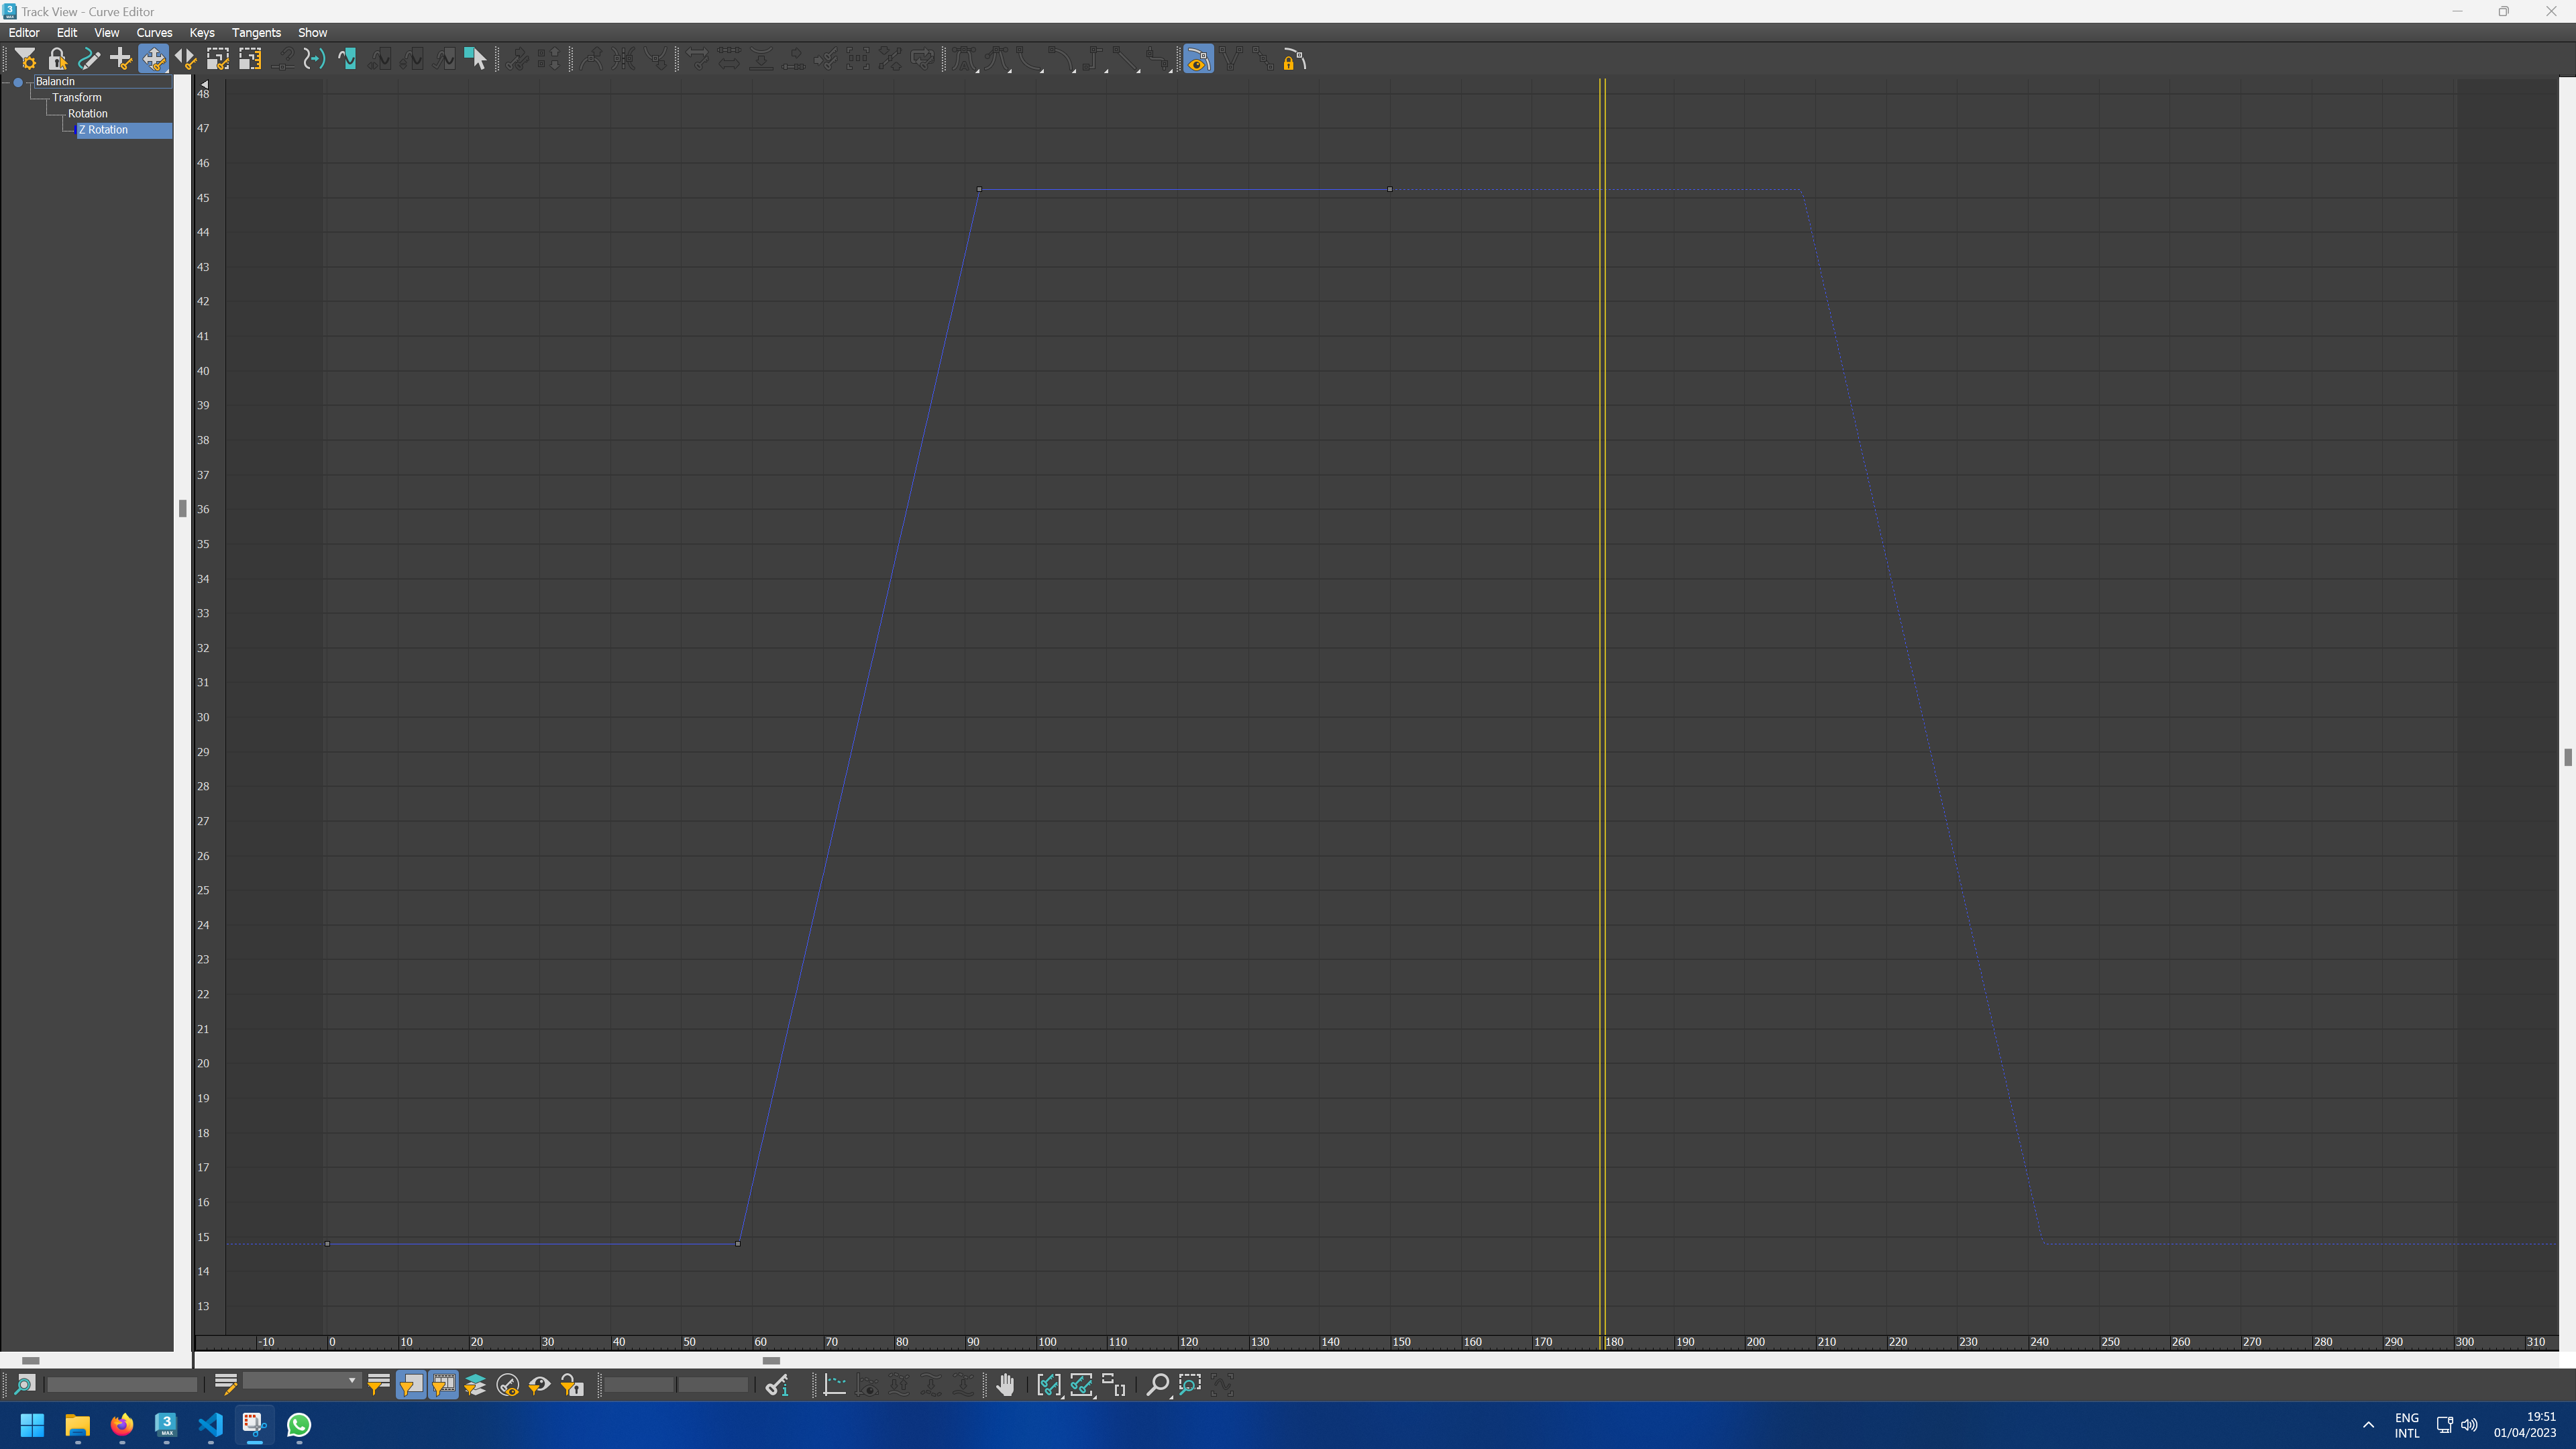
\includegraphics[width=\textwidth]{imagenes/curvas/Trampolin/blue.png}
    \caption{Curva que representa la rotación en el eje Z con respecto al tiempo.}
 \end{figure}

 Al igual que las pelotas, como el balancín es hijo del punto de apoyo, la rotación realmente se ve reflejada en el eje Y en coordenadas del mundo, ya que el padre actua de manera similar a los \textit{dummies}. Al igual que estos, el trampolín tiene utiliza una curva lineal, ya que la energia potencial de la pelota que se encuentra en el aire, al tocar el trampolin se la transfiere, sin la posibilidad de que acelere poco a poco.
\section{Iluminación de la escena}
Para la iluminación de la escena he utilizado una combinación de 3 luces, como se pedia en el guion, y de un cambio del color de fondo para que las zonas que no son iluminadas sean visibles.

\bigskip

Voy a dividir en subsecciones las explicaciones del color de fondo y de la iluminación:

\subsection{Color de fondo}

% rescribir
El color de fondo por defecto que tienen las escenas es el negro, haciendo que cuando se utiliza iluminacion, las zonas no iluminadas por los puntos de luz aparezcan negros por completo. Para solucionar esto es necesario modificar el color de fondo por un gris oscuro, para que se pueda ver toda la escena.

\bigskip

Para realizar esto hay que seguir los siguientes pasos:

% rescribir
En los menús de arriba, hace falta darle click a ``Rendering'' $\rightarrow$ ``Environment''.

% foto de eso

Se abrirá una ventana a la que hay que darle al rectángulo de selección de color de la sección ``Background'' y elegir un tono más claro.


% foto de mi tono

\subsection{Puntos de luz de la escena}
% rescribir
Para la iluminación de la escena he utilizado 3 \textit{Target Lights} junto a una distribución de luz de tipo \textit{Spotlight}, permitiendome modificar el cono de luz para que solo ilumine las bases, para el caso de las luces de los extremos, y el trampolín, para el caso de la luz intermedia.

% foto de los conos

Ahora bien, los \textit{keyframes} para el foco de la izquierda son:

\begin{itemize}
    \item \textbf{Instante 0: }No hay ningún cambio de ningún tipo, es para hacer que la animación de ping-pong funcione bien y para ver los rebotes previos que realiza la bola. La luz ahora mismo se ecneutnra encendida y de color blanco.
    \item \textbf{Instante 38: }La luz se encuentra exactamente igual que en el instante anterior.
    \item \textbf{Instante 58: }La luz pasa a tener color rojo y apagarse (intensidad a 0) porque la pelota ha saltado de la plataforma.
    \item \textbf{Instante 150: }Exactamente igual que en el instante anterior. Se realiza para hacer que la animación inversa funcione bien y porque la pelota no esta en la base.
\end{itemize}

Las curvas de animación son las isguientes:

\begin{figure}[H]
    \centering
    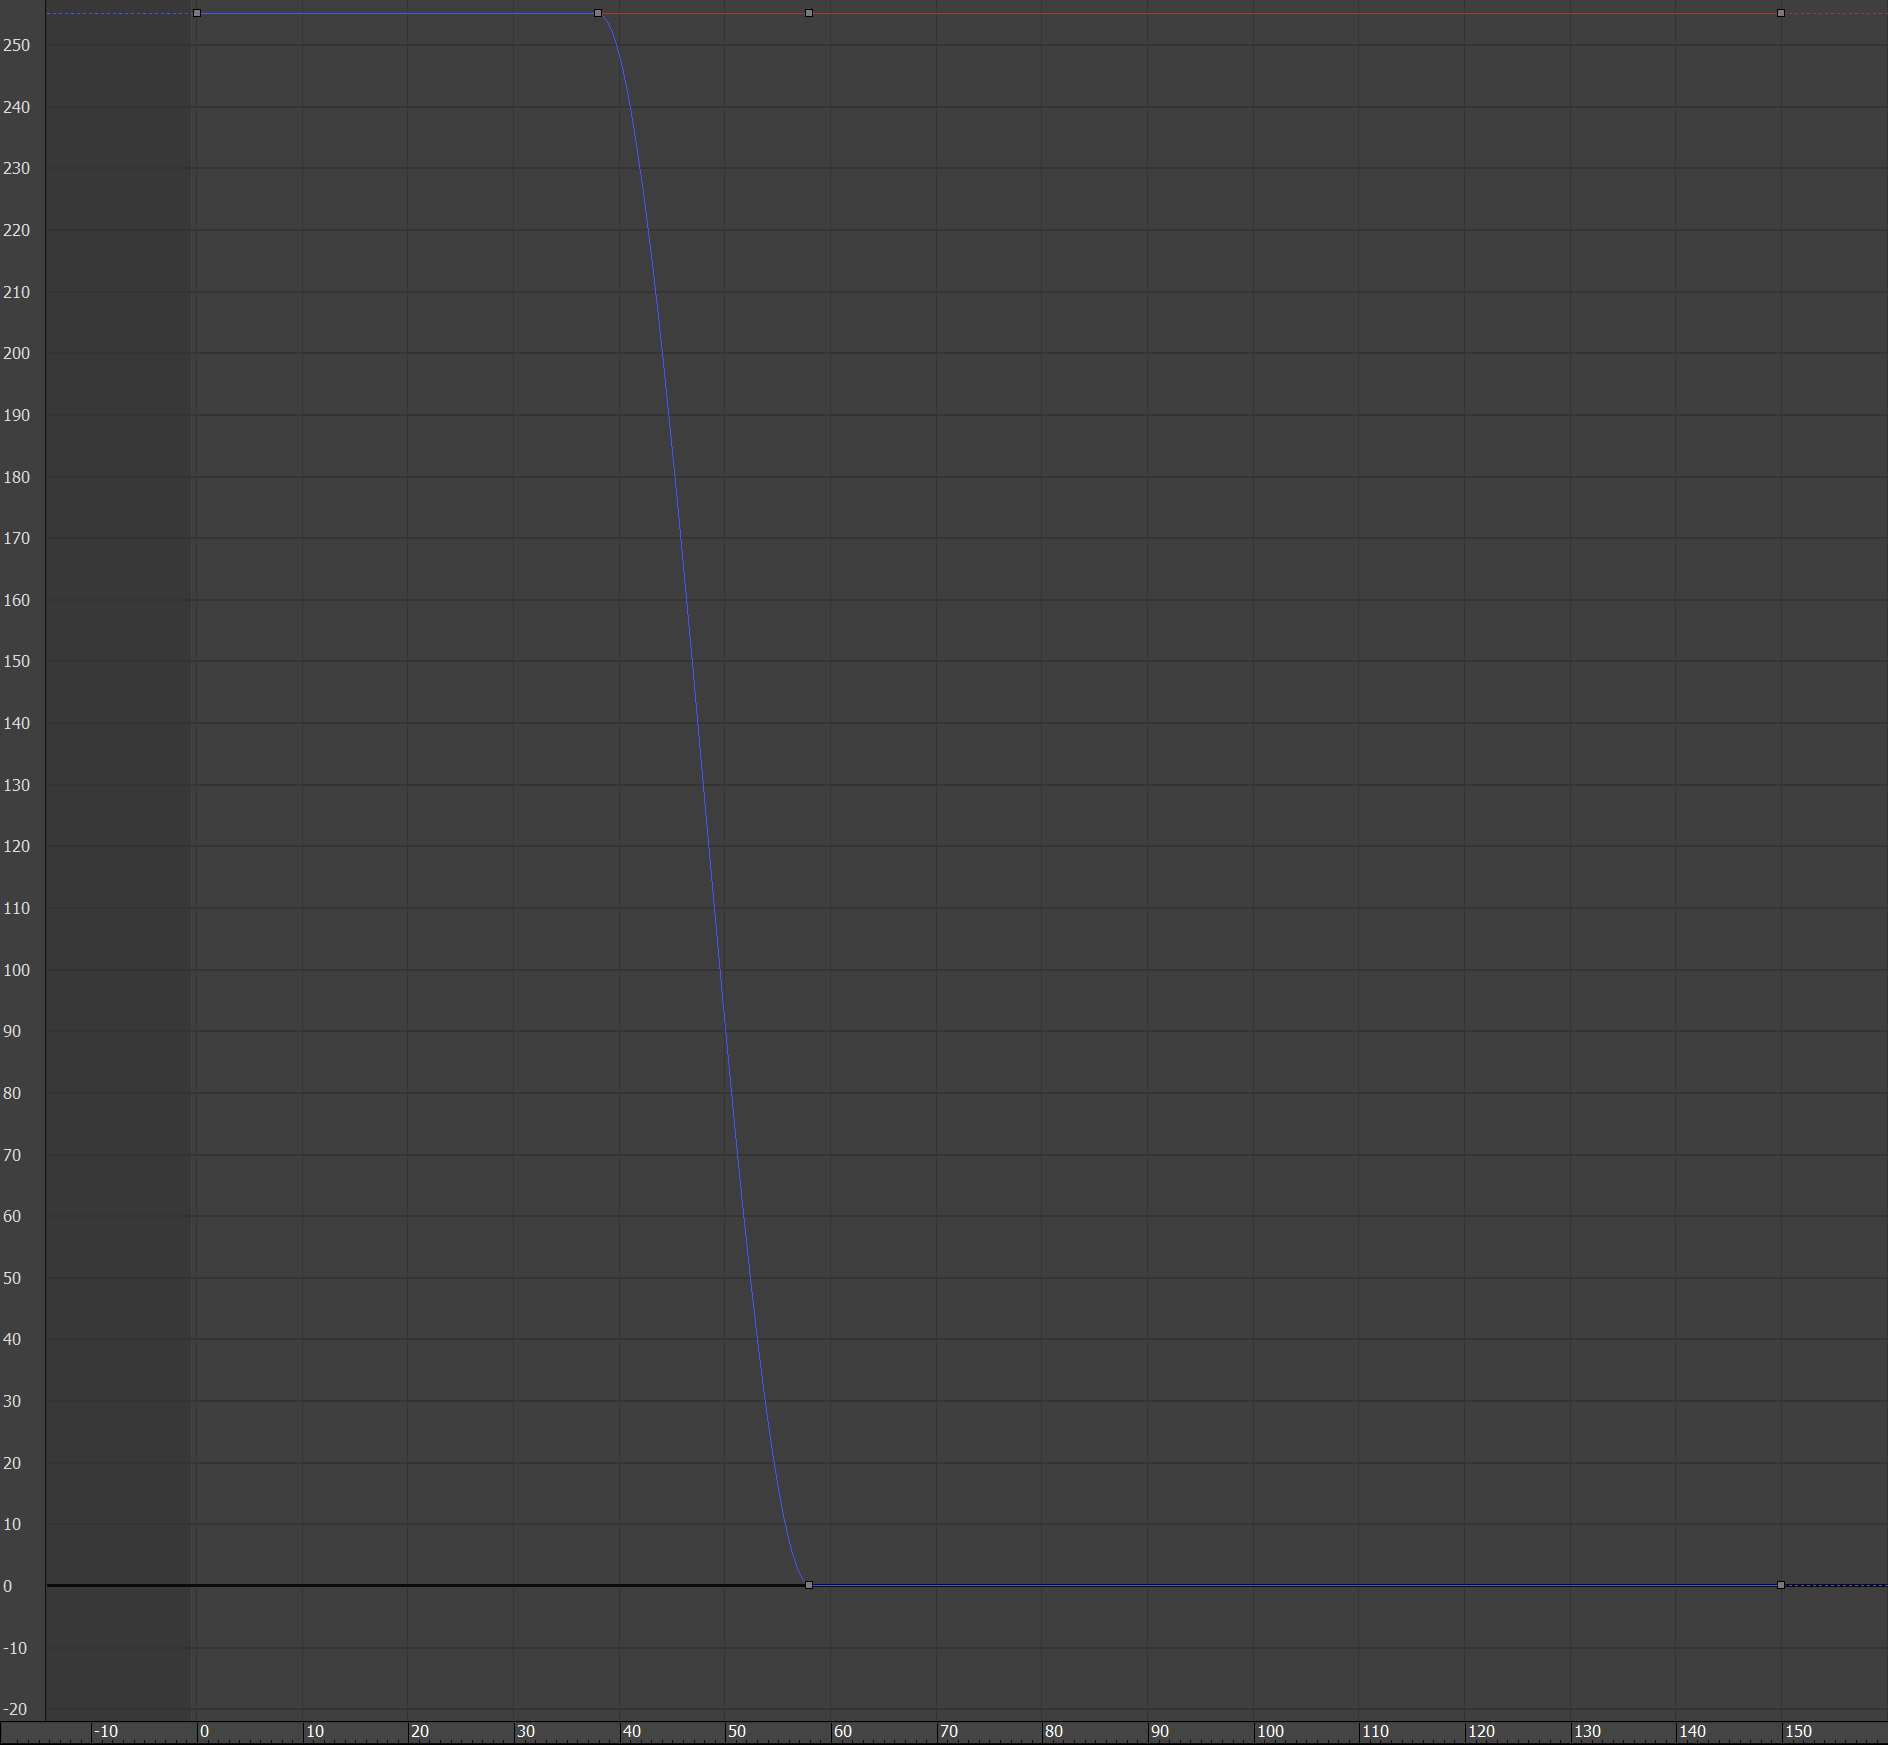
\includegraphics[width=\textwidth]{imagenes/curvas/LL/filter.png}
    \caption{Curva que representa el color de la luz con respecto al tiempo.}
 \end{figure}

En la curva he usado una función \textit{Slow-in/Slow-out} para simular la iluminación progresiva que tendría una luz incandescente al ser encencidad y apagada.

 \begin{figure}[H]
    \centering
    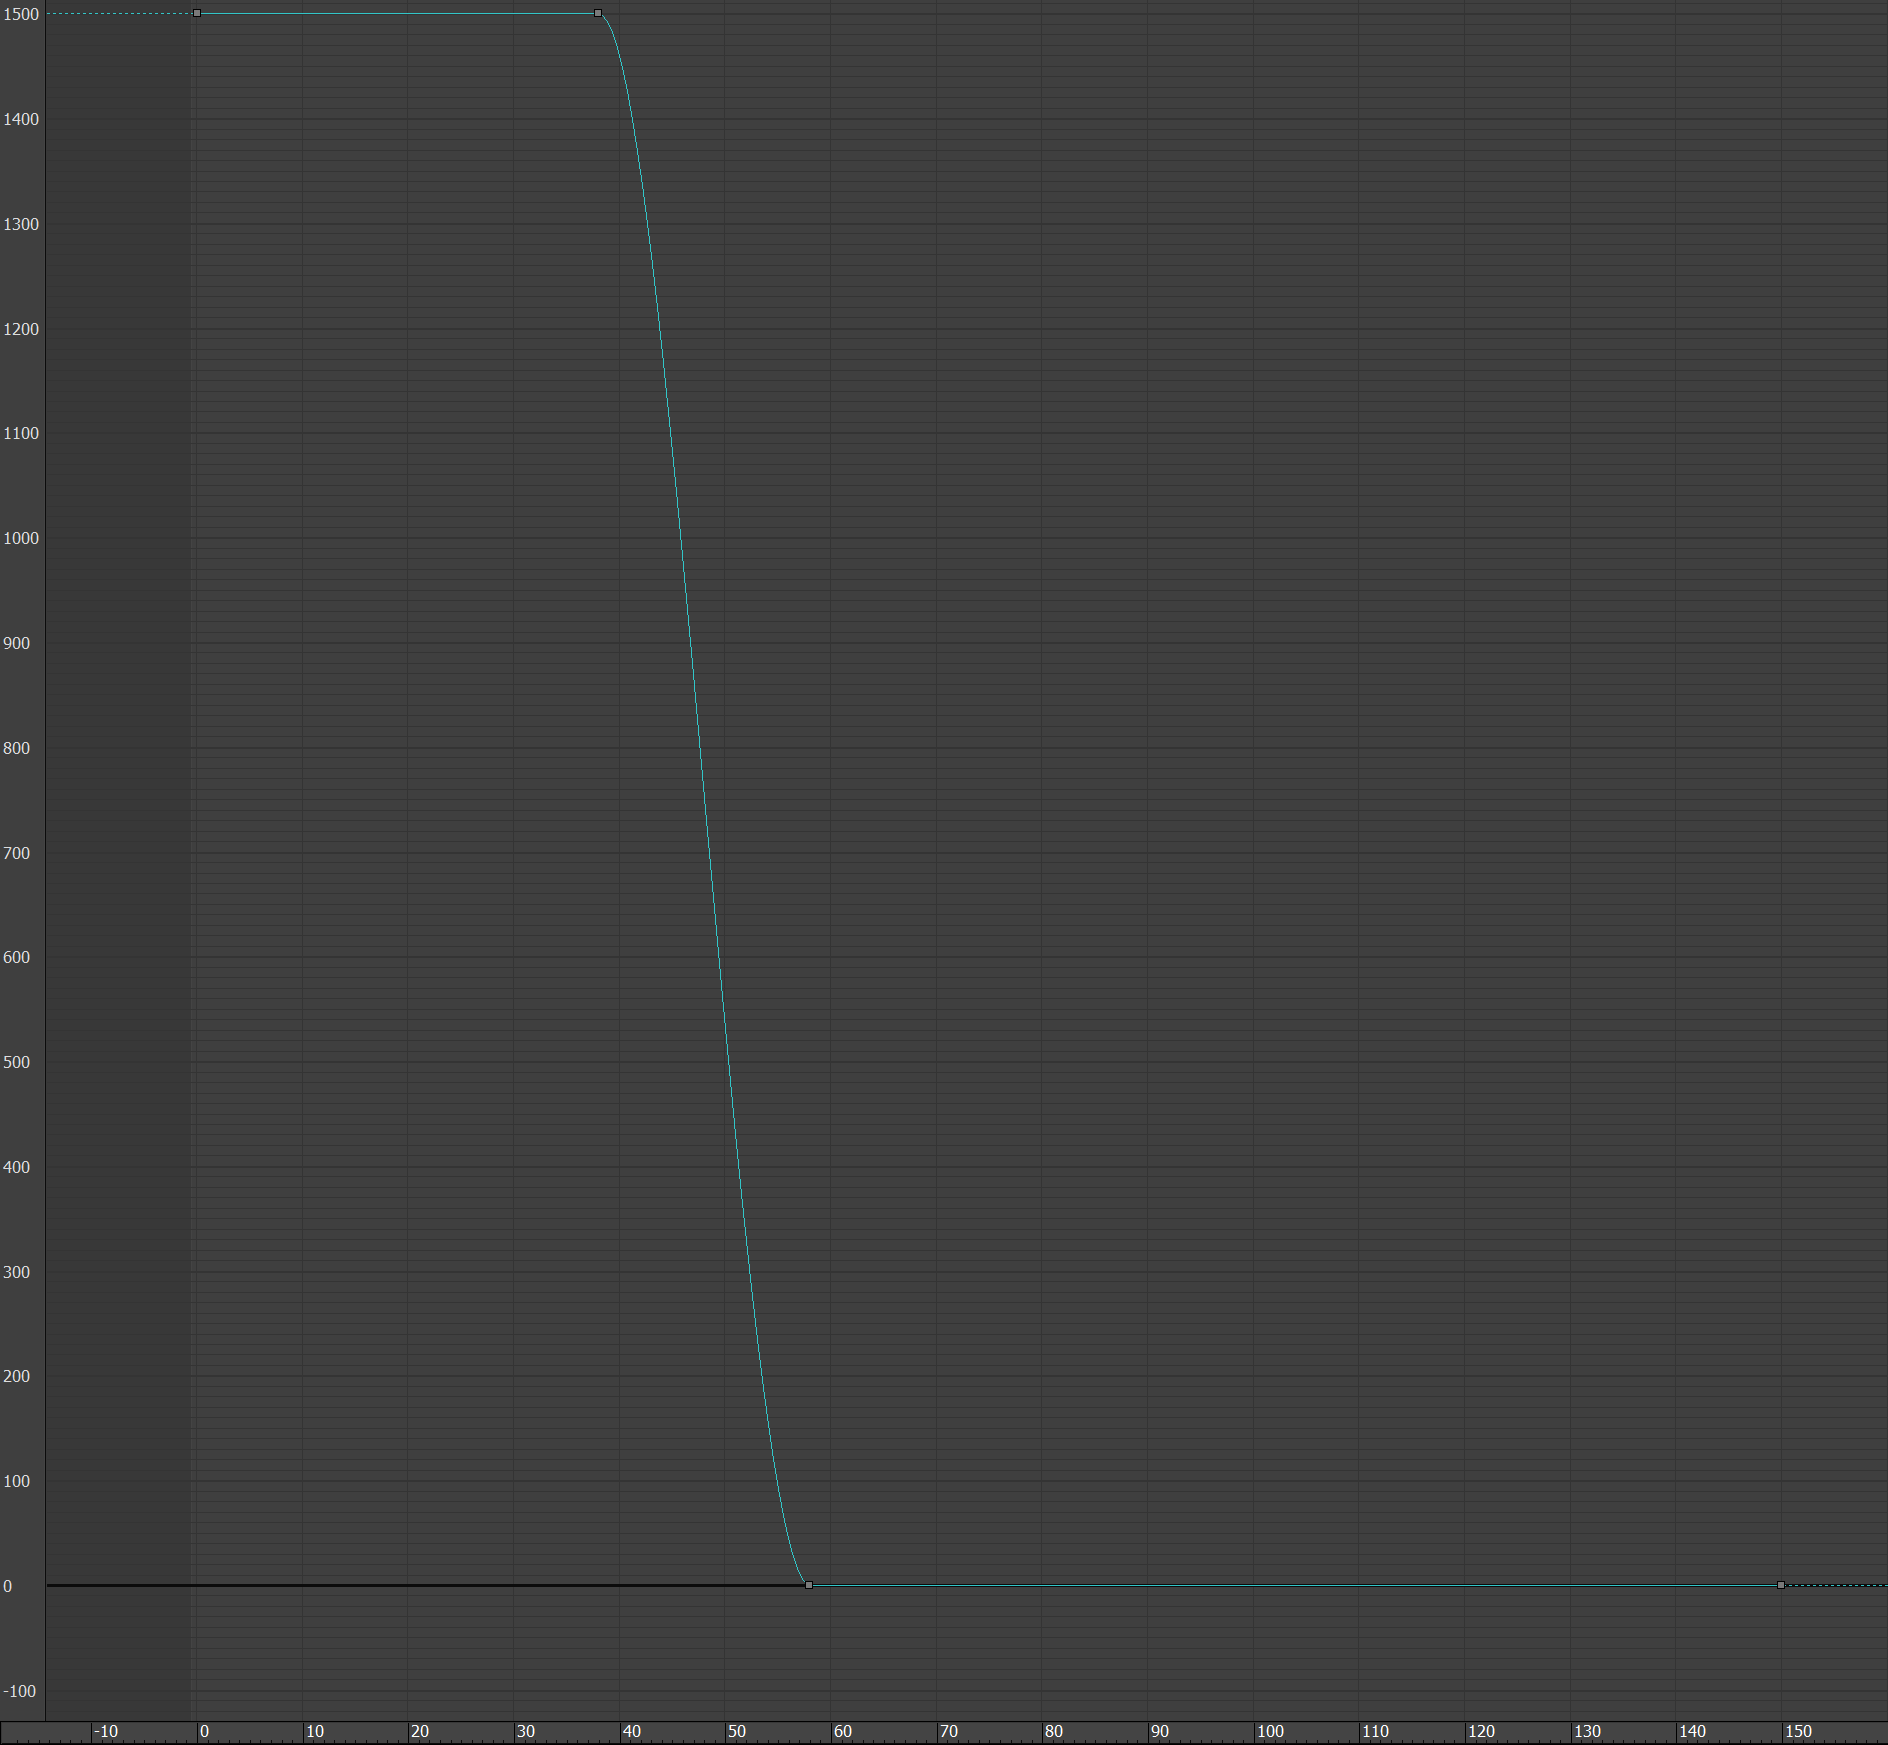
\includegraphics[width=\textwidth]{imagenes/curvas/LL/intensity.png}
    \caption{Curva que representa la intensidad de la luz con respecto al tiempo.}
 \end{figure}

 En esta curva también he usado el mismo tipo de función que en la anterior, con el objetivo de simular el encendido y apagado progresivo que tienen algunas luces, entre ellas las incandescentes como antes.

 \bigskip

 El punto de luz del otro extremo que ilumina la otra pelota tiene los mismos \textit{keyframes}, pero comenzando desde el final:

 \begin{itemize}
    \item \textbf{Instante 0: }Se encuentra de color rojo y con la intensidad a 0. Esto se hace para que la animación inversa funcione de manera correcta con las demás componentes y porque no se encuentra la pelota en la base.
    \item \textbf{Instante 92: }La luz sigue exactamente igual que en el instante anterior.
    \item \textbf{Instante 112: }La luz ahora se encuentra iluminada al maximo y de color blanco.
    \item \textbf{Instante 150: }Se enceuntra exactamente igual que en el instante anterior, con el objetivo de que la animación inversa funcione correctamnet y porque la pelota esta rebotando en la base.
 \end{itemize}
 
Las curvas de animación osn las isuignetes:

\begin{figure}[H]
    \centering
    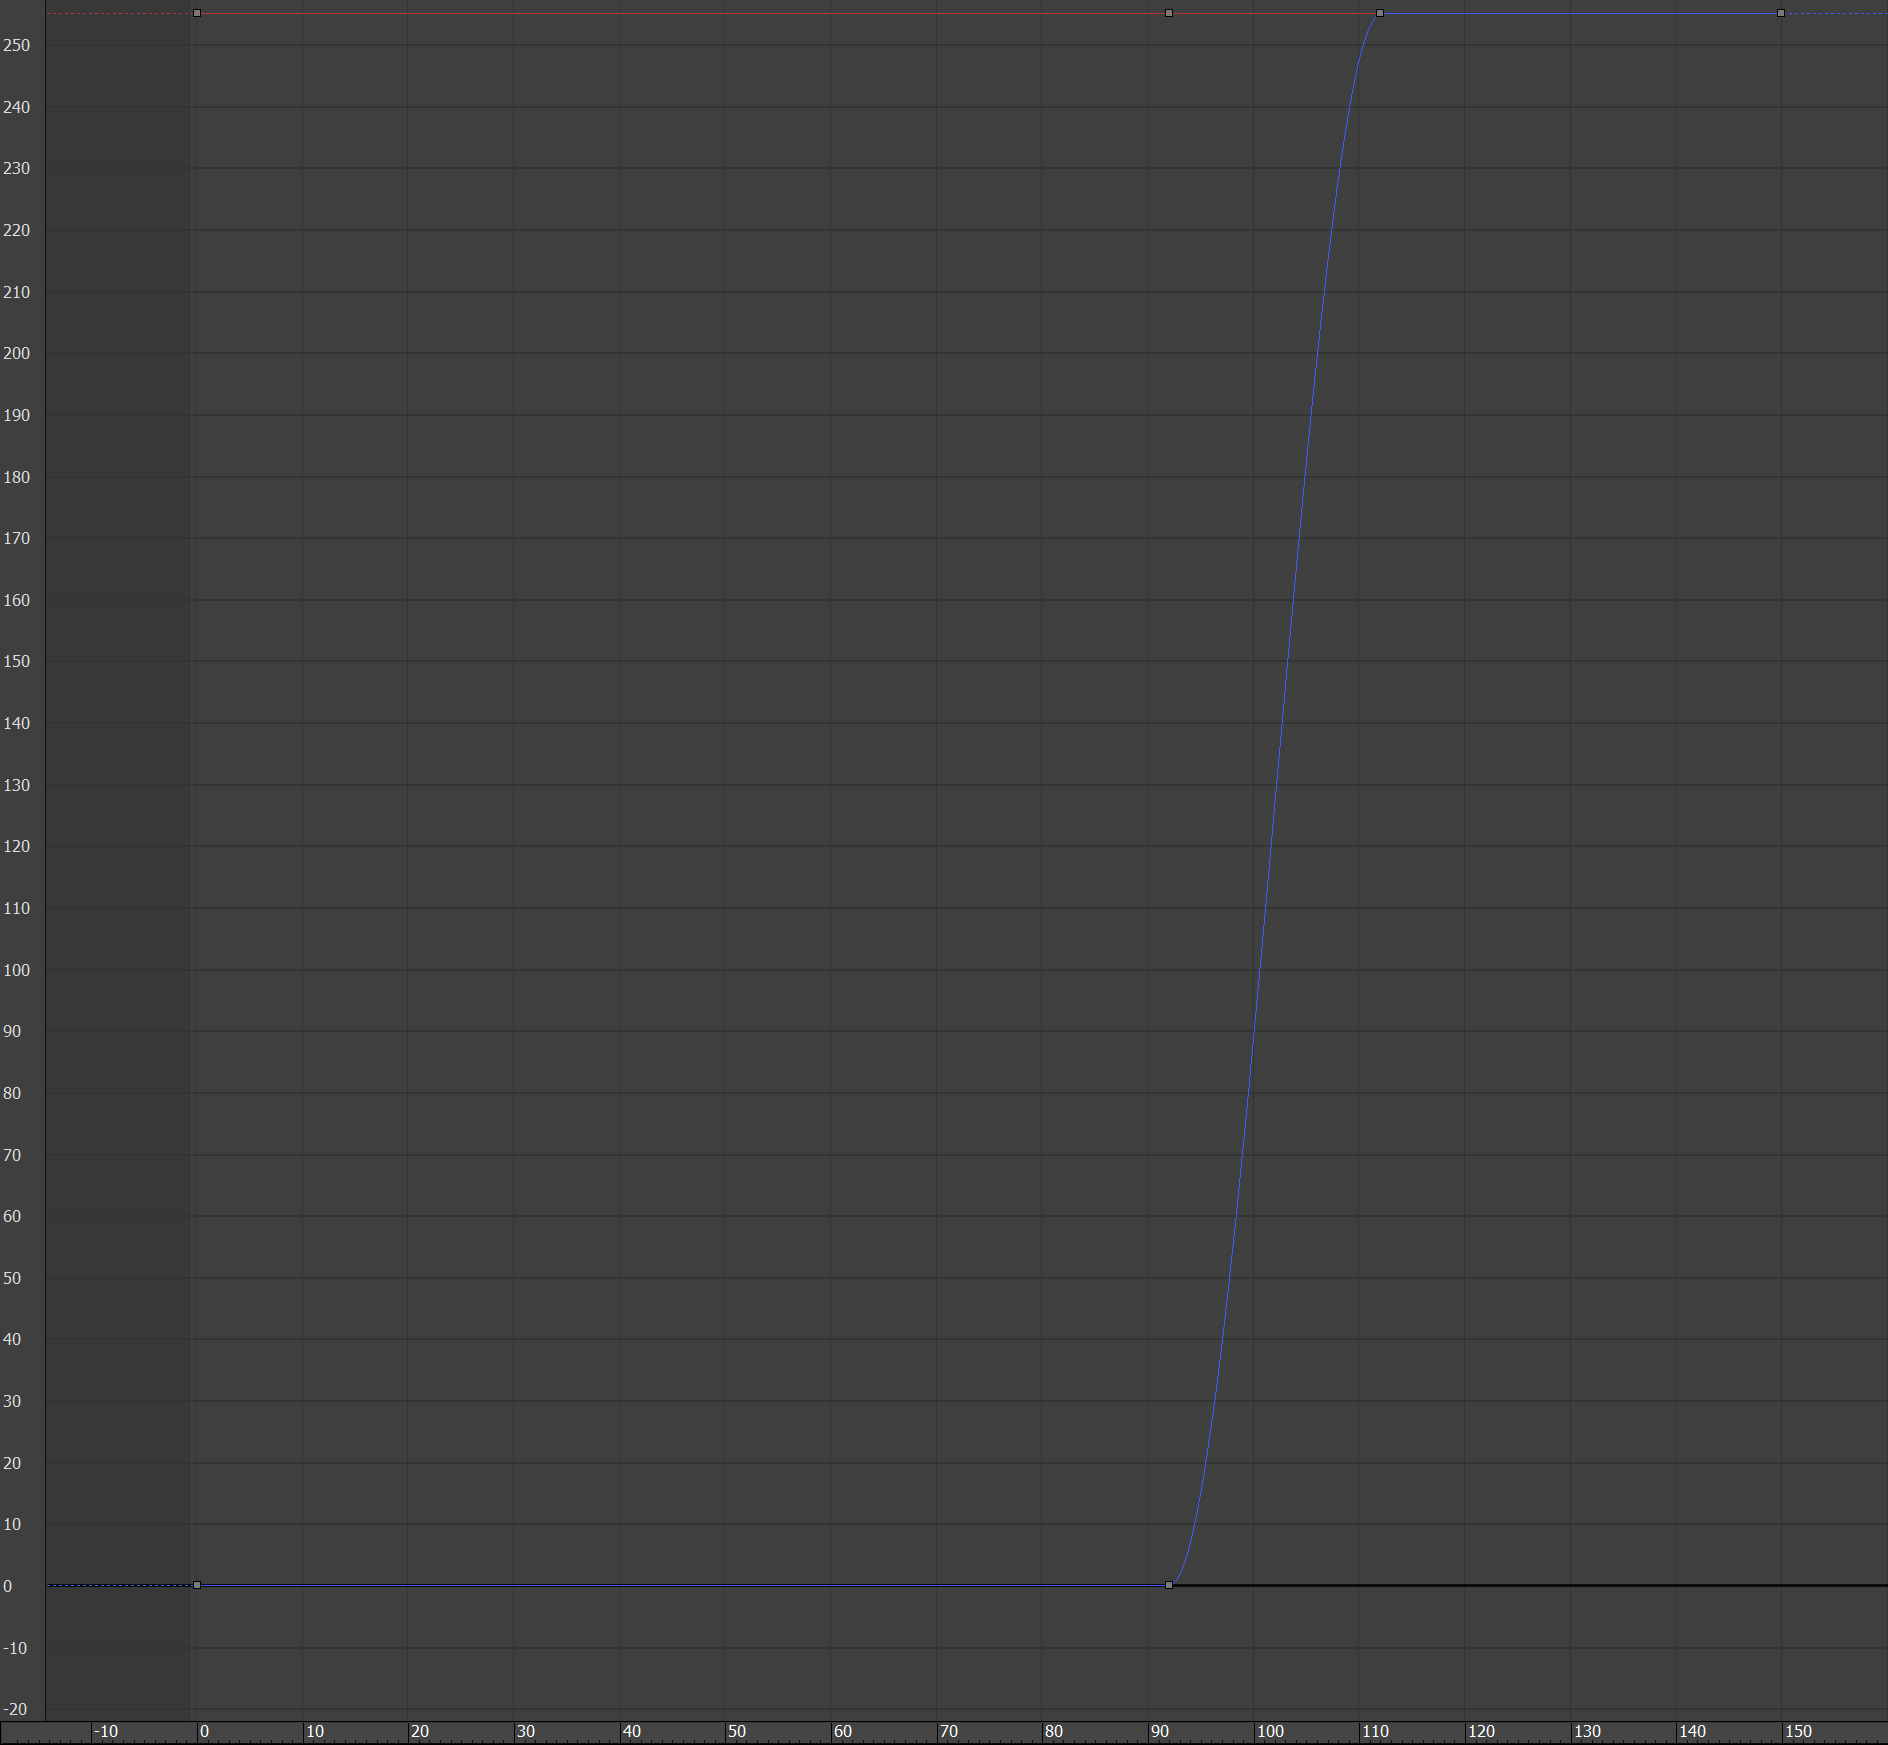
\includegraphics[width=\textwidth]{imagenes/curvas/LR/filter.png}
    \caption{Curva que representa el color de la luz con respecto al tiempo.}
 \end{figure}

 \begin{figure}[H]
    \centering
    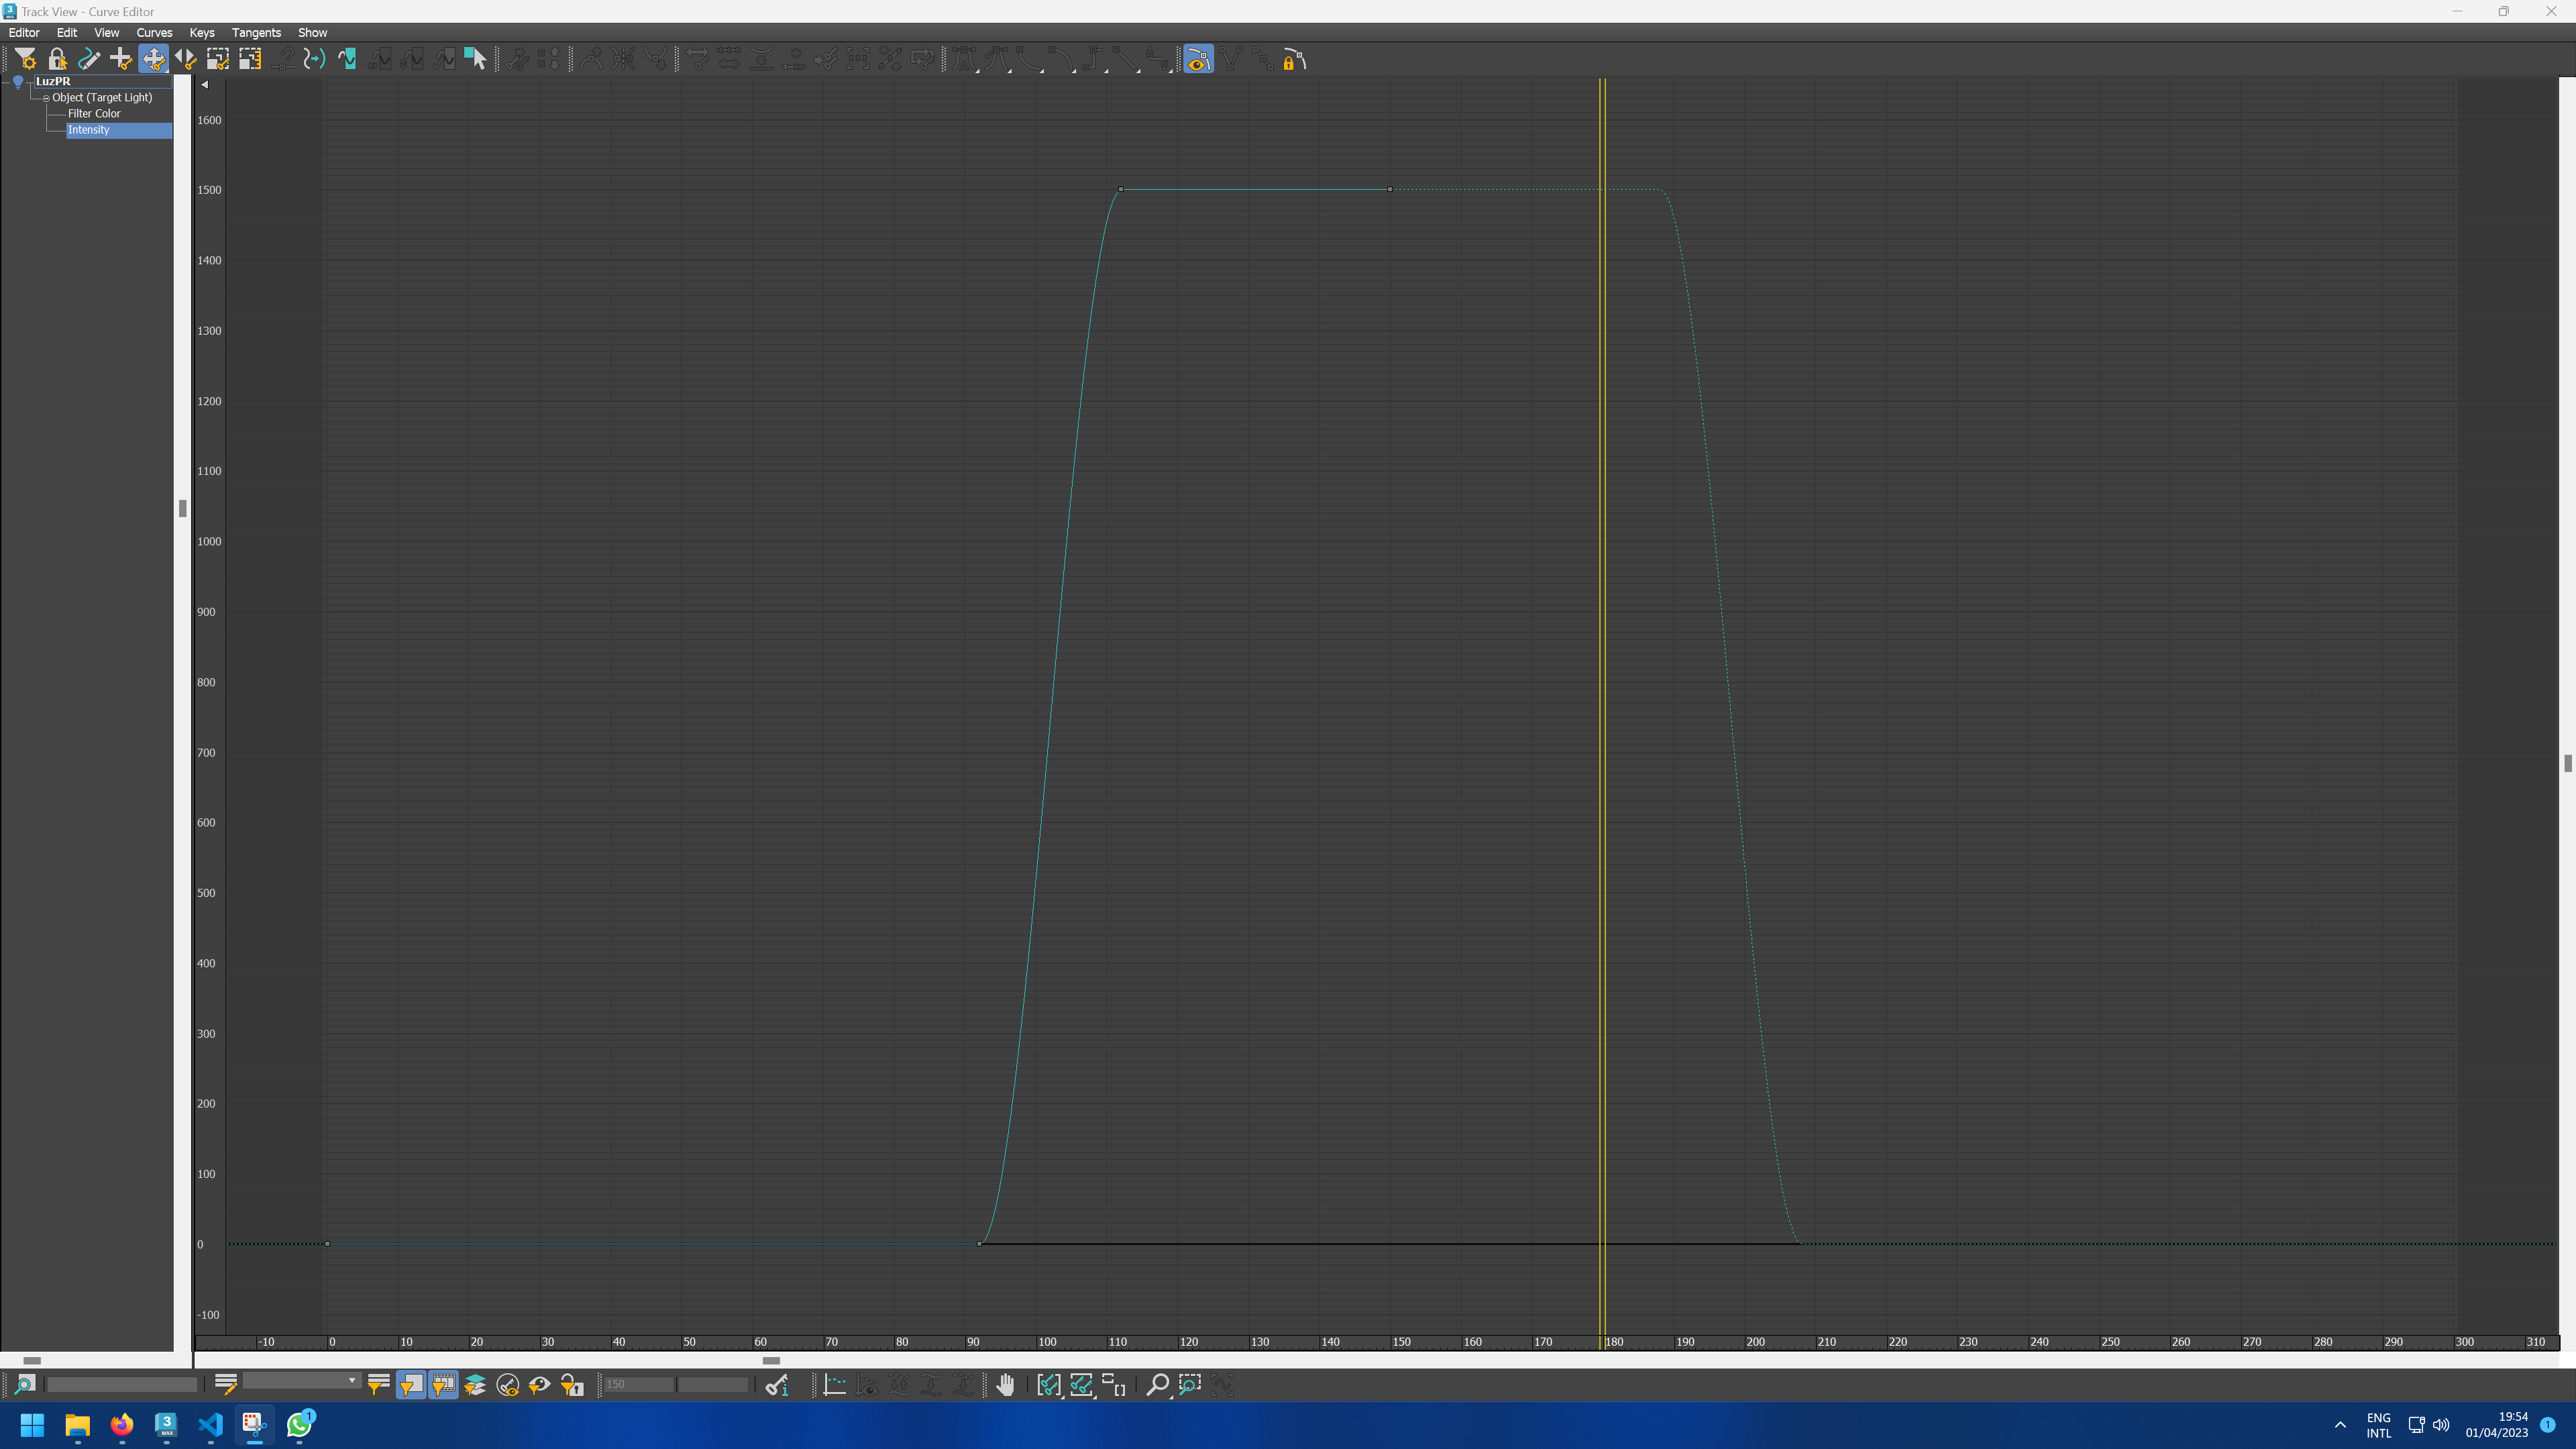
\includegraphics[width=\textwidth]{imagenes/curvas/LR/intensity.png}
    \caption{Curva que representa la intensidad de la luz con respecto al tiempo.}
 \end{figure}

Al igualq ue con la luz del otro extremo, esta se encenderá y apagará progresivamente, simulando una luz incandescente.


Por último, la luz intermedia, utilizada para iluminar el trampolín, tiene los siguientes \textit{keyframes}:

\begin{itemize}
    \item \textbf{Instante 0: }La luz se encuentra apagada y de color rojo, para hacer la animacion inversa correctamente y porque no hay movimiento en el trmapolin.
    \item \textbf{Instante 38: }La luz sigue exactamente igual que en el isntante anterior.
    \item \textbf{Instante 58: }La luz se encuentra encendida y de color blanco, indicando que hay movimiento en el tramploin.
    \item \textbf{Instante 92: }La luz sigue exactamente igual que antes, ya que todavia hay movimiento en el trampolin.
    \item \textbf{Instante 112: }La luz ahora se encuentra apagada y de color rojo, al no haber más movimiento en el trampolin.
    \item \textbf{Instante 150: }Sigue sin haber movimiento, por lo que sigue apagada y de color rojo. Tambien es para que la animacion inversa funcione.
\end{itemize}

Y las curvas de animacion son:

\begin{figure}[H]
    \centering
    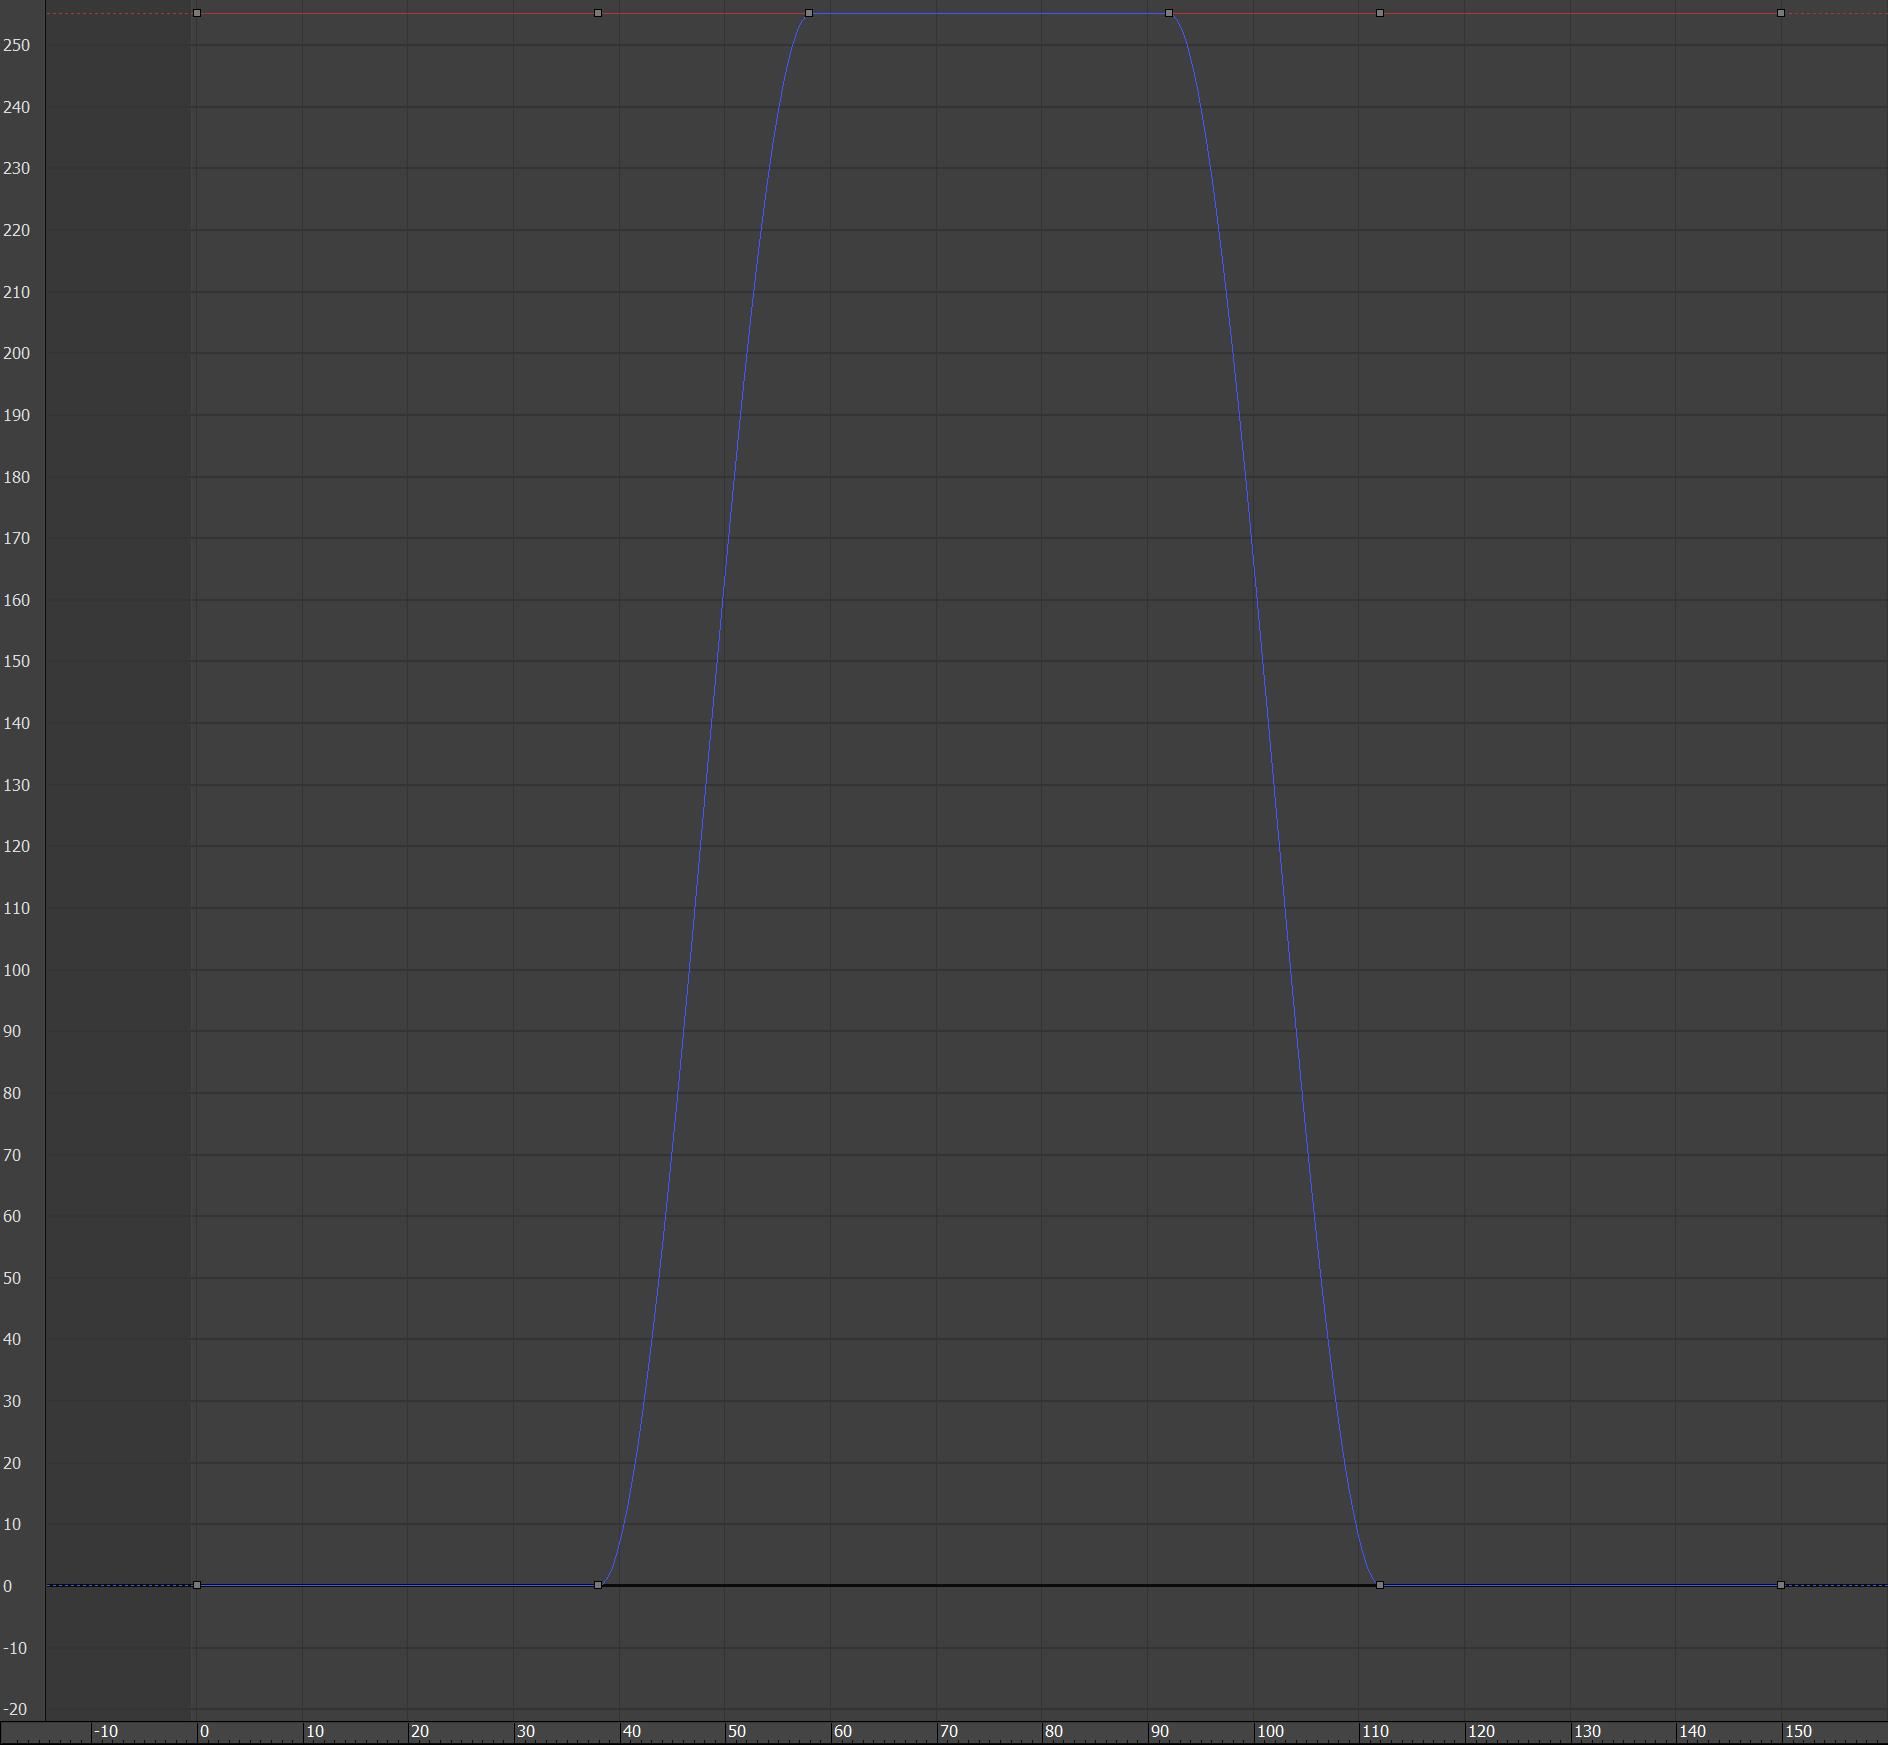
\includegraphics[width=\textwidth]{imagenes/curvas/LC/filter.png}
    \caption{Curva que representa el color de la luz con respecto al tiempo.}
 \end{figure}

 \begin{figure}[H]
    \centering
    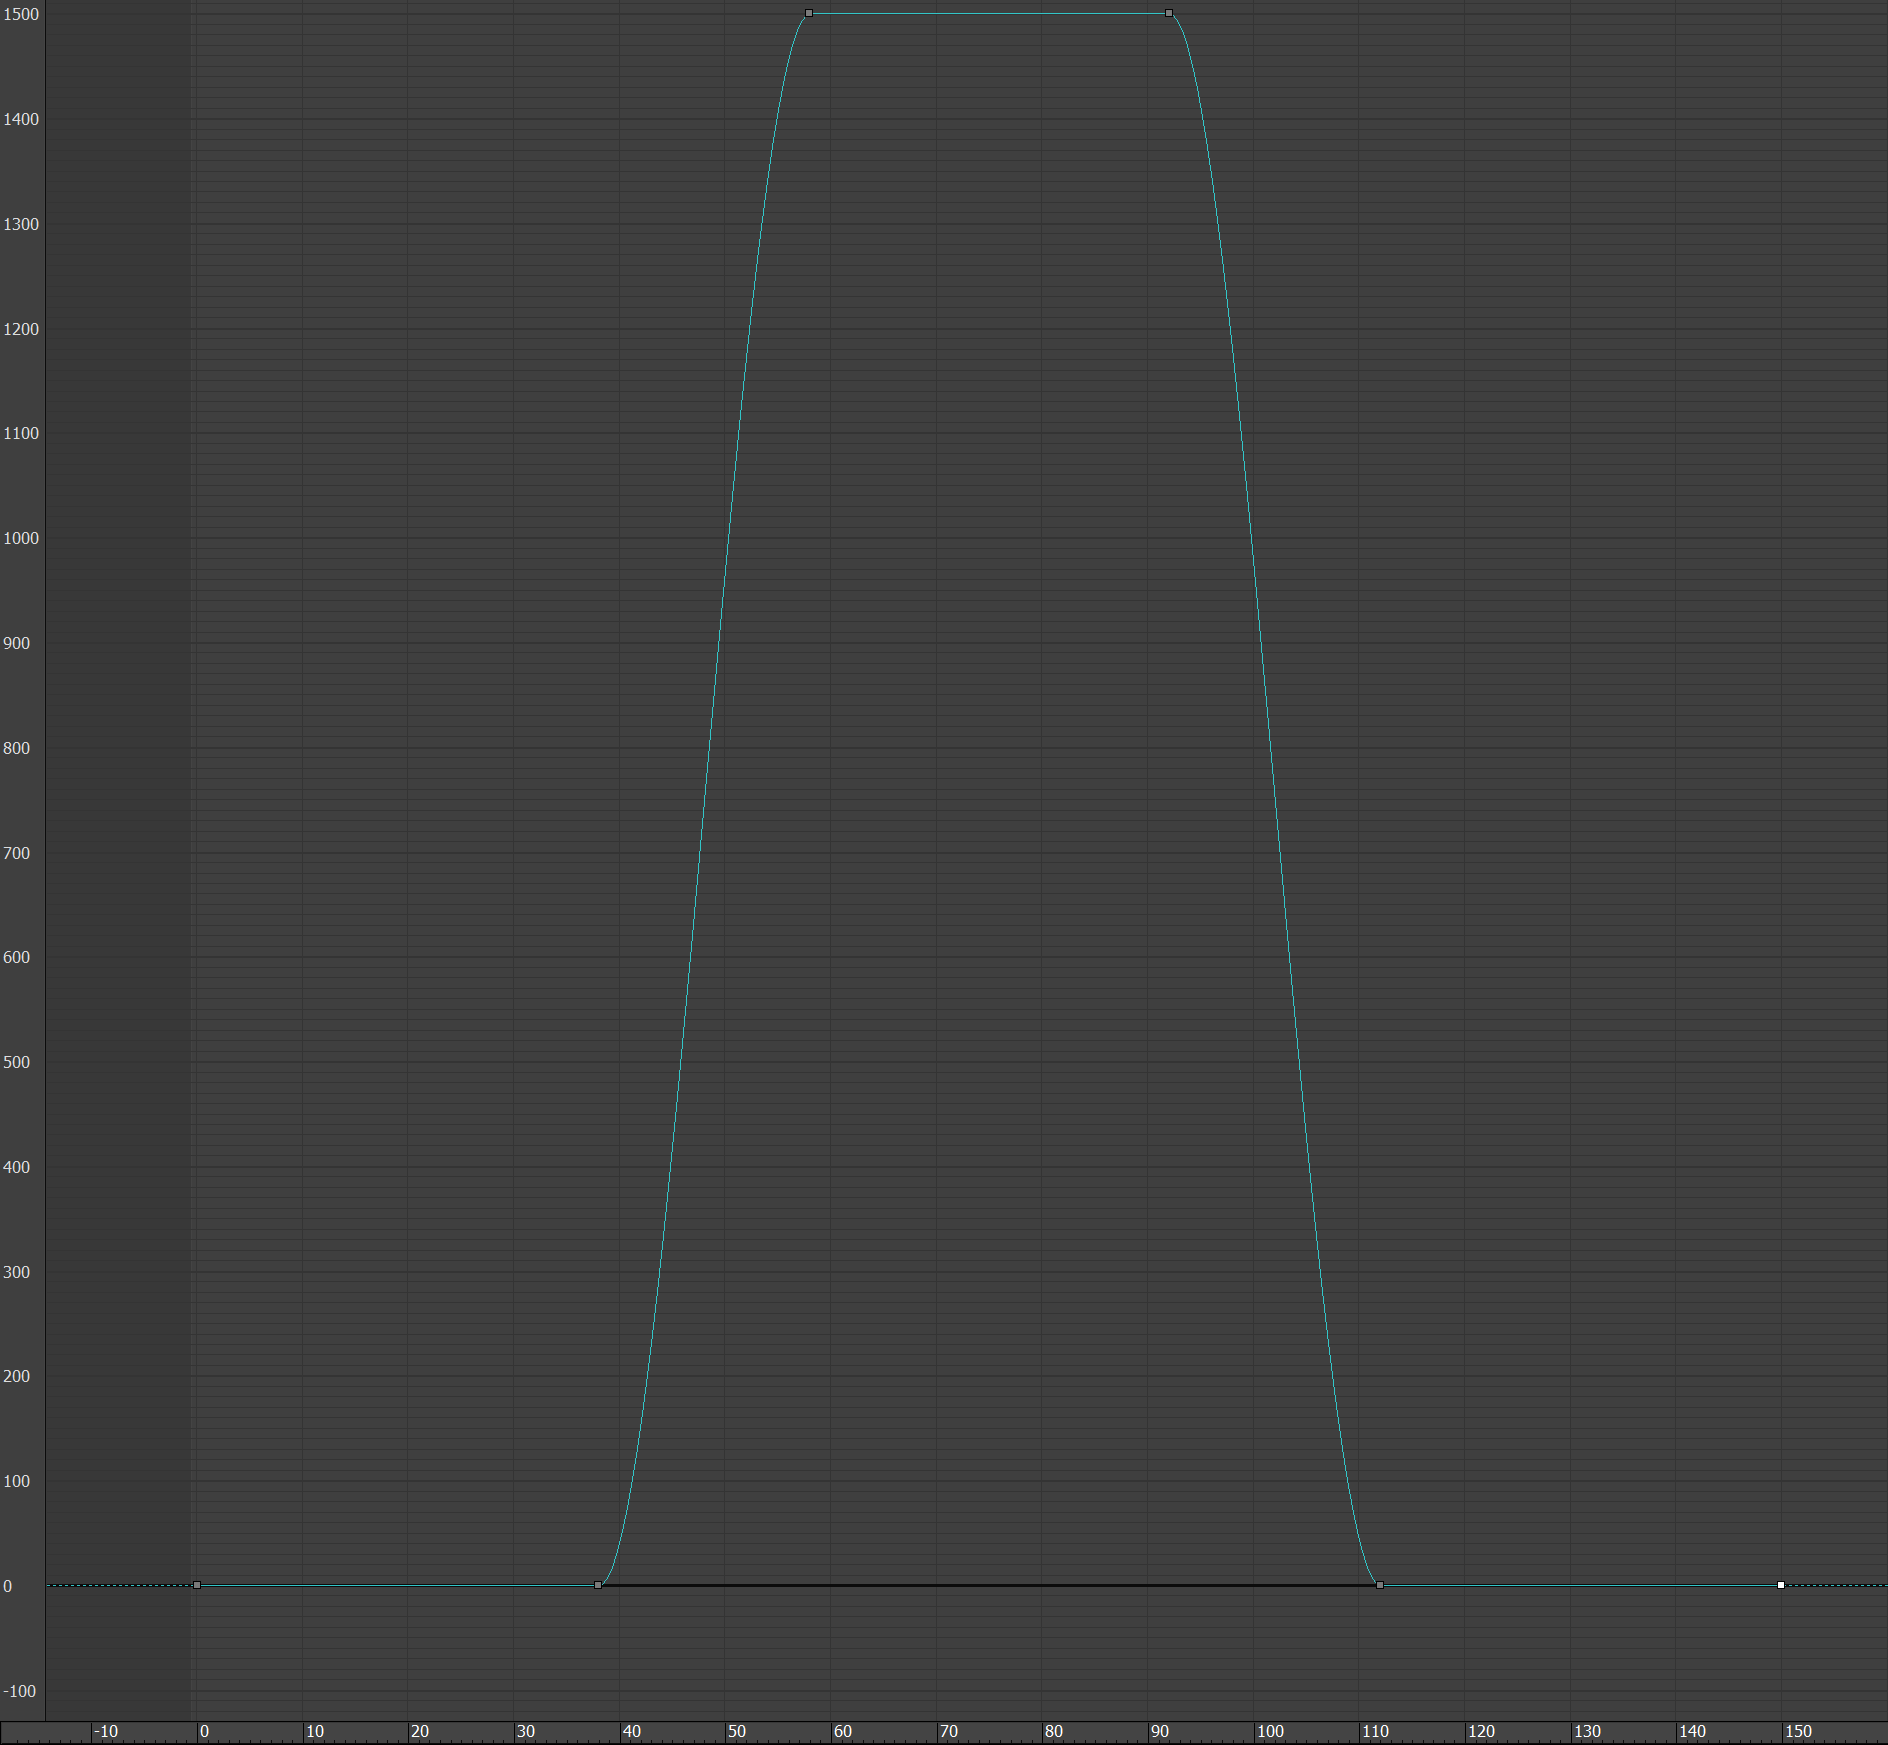
\includegraphics[width=\textwidth]{imagenes/curvas/LC/intensity.png}
    \caption{Curva que representa la intensidad de la luz con respecto al tiempo.}
 \end{figure}

Al igual que con las otras luces, he utilizado una curva \textit{Slow-in/Slow-out} para simular el encendido y apagado progresivo de la luz.

\section{Animación de la cámara}

\section{Animación final}

\end{document}
